\documentclass[a4paper,12pt]{report}
\usepackage{alltt, fancyvrb, url}
\usepackage{graphicx}
\usepackage[utf8]{inputenc}
\usepackage{float}
\usepackage{hyperref}
\usepackage[italian]{babel}
\usepackage[italian]{cleveref}
\usepackage{xcolor}
\usepackage[dvipsnames]{xcolor}
\usepackage{array}
\title{Relazione su "Daidokoro" \\ Elaborato per il corso di Basi di Dati}

\author
{
    Matteo Giorgini - 0001136576 \\
    Tommaso De Tommaso - 0001077338 \\
    Edoardo Scorza - 0001077424 \\
}
\date{\today}
\begin{document}
\maketitle
\tableofcontents

\chapter{Analisi dei requisiti}
\section{Requisiti in linguaggio naturale}
Si vuole realizzare un database a supporto di un social network di ricette, questo dovrà tenere traccia degli \textbf{\textit{utenti}} registrati salvandone il loro username, la foto profilo, l'email, la password ed un codice univoco per identificarli.
Inoltre, si vuole anche tenere traccia dell'esperienza e del livello, i quali rappresentano il progresso di un utente nello sblocco di \textbf{\textit{obiettivi}} che sono caratterizzati da un nome, una descrizione e dalla quantità di esperienza da dare all'utente una volta sbloccato.
Questi vengono usati per incitare l'utente ad utilizzare tutte le diverse funzionalità del software, che possono anche essere limitate fino allo sblocco di un determinato obiettivo.
L'utente, dopo aver effettuato l'accesso, potrà osservare le ricette altrui, aggiungerle ai preferiti, salvarle in collezioni o in diete e valutarle con un voto ed un commento.
L'utente potrà anche pubblicare le proprie \textbf{\textit{ricette}} inserendone il nome, la foto, la descrizione, la difficoltà e il tempo di realizzazione indicativo, oltre agli ingredienti che la compongono ed ai passi necessari a prepararla.
Gli \textbf{\textit{ingredienti}} sono composti da un nome, una descrizione, dai valori nutrizionali e dalla categoria nutrizionale a cui appartengono.
Le \textbf{\textit{collezioni}} possiedono un nome, una descrizione, la data di creazione e la lista di ricette che ne fanno parte.
Ci sono anche le diete, che funzionano come le collezioni, ma differiscono nel fatto che devono aderire ad una categoria nutrizionale specifica, vincolando quindi le ricette che si possono aggiungere.
Infine, le \textbf{\textit{valutazioni}} che gli utenti possono lasciare a ricette, collezioni o diete, consistono in un voto positivo o negativo, eventualmente accompagnato da un commento se l'utente ha sbloccato l'apposito obiettivo.
\\
\section{Analisi ed estrazione dei concetti}
Il testo dei requisiti fornisce una accurata descrizione delle entità chiave, tuttavia è anche abbastanza ambigua sulla gestione dei vincoli generati dagli obiettivi, su dove memorizzare i valori nutrizionali degli ingredienti ed sui vincoli delle diete che accettano solo ricette con ingredienti di una certa categoria nutrizionale.
\\\\
Molti dei vincoli funzionali che dipendono dallo sblocco di un obiettivo non sono modellabili nel database e quindi saranno implementati nella programmazione, tuttavia per differenziare tra la valutazione senza commento e quella con il commento, si modifica l'entità valutazione spostando il commento in un suo subset denominato \textbf{\textit{critica}}.
I \textbf{\textit{valori nutrizionali}} saranno memorizzati in una tabella separata che avrà una relazione 1 a 1 con la tabella degli ingredienti in modo da separare meglio dati non essenziali che non identificano direttamente l'ingrediente. Infine, le \textbf{\textit{diete}} sono un particolare tipo di collezione e quindi le si trasformano in un subset.
\begin{table}[h!]
    \centering
    \begin{tabular}{ |p{1.2in}|p{1.2in}|p{2.4in}| }
        \hline
        \scriptsize{\textbf{Nome}} & \scriptsize{\textbf{Tipologia}} & \scriptsize{\textbf{Descrizione}} \\
        \hline
        \scriptsize{Utente} & \scriptsize{Entità} & \scriptsize{-} \\
        \hline
        \scriptsize{Obiettivo} & \scriptsize{Entità} & \scriptsize{-} \\
        \hline
        \scriptsize{Ricetta} & \scriptsize{Entità} & \scriptsize{-} \\
        \hline
        \scriptsize{Ingrediente} & \scriptsize{Entità} & \scriptsize{-} \\
        \hline
        \scriptsize{Valore nutrizionale} & \scriptsize{Entità minore} & \scriptsize{-} \\
        \hline
        \scriptsize{Collezione} & \scriptsize{Entità} & \scriptsize{-} \\
        \hline
        \scriptsize{Dieta} & \scriptsize{Entità \newline \textit{Subset di Collezione}} & \scriptsize{-} \\
        \hline
        \scriptsize{Valutazione} & \scriptsize{Entità} & \scriptsize{-} \\
        \hline
        \scriptsize{Critica} & \scriptsize{Entità \newline \textit{Subset di Valutazione}} & \scriptsize{-} \\
        \hline
        \scriptsize{Categoria nutrizionale} & \scriptsize{Entità} & \scriptsize{-} \\
        \hline
    \end{tabular}
    \caption{Entità e relazioni principali}
\end{table}

\chapter{Progettazione concettuale}
Per la progettazione concettuale abbiamo considerato diverse cose,
tra cui, la organizzazione della applicazione e le capacità degli utenti,
in primis, la app è di tipo client-server, quindi il database è unico e
possiede tutti i dati del "ecosistema"(client e server), gli utenti sono potenzialmente tanti
e hanno un frequente accesso al database, motivo per il cui i dati sono
frammentati, separati in varie parti, per evitare un accesso non essenziale a grandi quantità di dati, e ridurre il carico sul database.    
\section{Schema scheletro}
\begin{figure}[H]
    \centering
   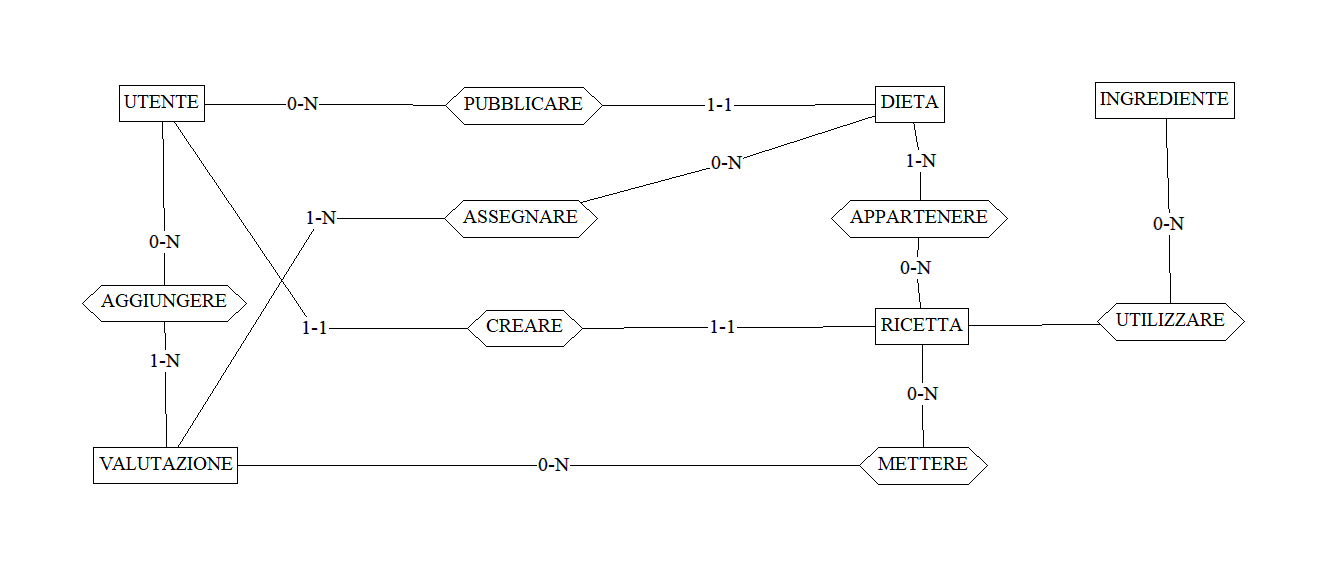
\includegraphics[width=0.9\textwidth]{app_images/schema-scheletro.png}  
    \label{fig:example}
\end{figure}
La prima versione dello schema evidenzia gli elementi chiave 
che costruiscono le informazioni su cui si basa la applicazione:
\begin{itemize}
    \item Utente
    \item Ricetta
    \item Valutazione
    \item Ingrediente
    \item Dieta
\end{itemize}

\section{Raffinamenti proposti}
Analizzando meglio la possibile esperienza dell'utente
sono molte le possibili aggiunte, abbiamo cercato
dunque di rendere il database completo senza complicarlo eccessivamente:
\subsection{Dieta}
La dieta, corrisponde alla possibilità di raggruppare ricette
per rendere più significativo il significato di essa abbiamo deciso di 
imporre dei limiti, come la categoria, che limita la tipologia di ricette 
inseribili, la creazione di essa è permessa all'utente solo dopo aver sbloccato un determinato obiettivo.
\subsection{Collezione}
Per non limitare le possibilità dell'utente abbiamo deciso di creare 
una variante più generale della dieta, la collezione
essa permette di salvare ricette indiscriminatamente.
\subsection{Obiettivo}
Per Dare più autorevolezza agli utenti esperti e
filtrare utenti "troll" abbiamo deciso di implementare dei requisiti,
per fare delle diete bisogna aver sbloccato un obbiettivo, 
cosi per le critiche
\subsection{Valutazione}
Per le valutazioni abbiamo optato su 2 tipologie
valutazione e critica, la prima consiste in un voto
numerico, assegnabile da un utente generico, il secondo è una critica
che aggiunge il commento, questa limitata da un obbiettivo.


\section{Schema Concettuale}
Il risultato finale è questo schema:
\begin{figure}[H]
    \centering
    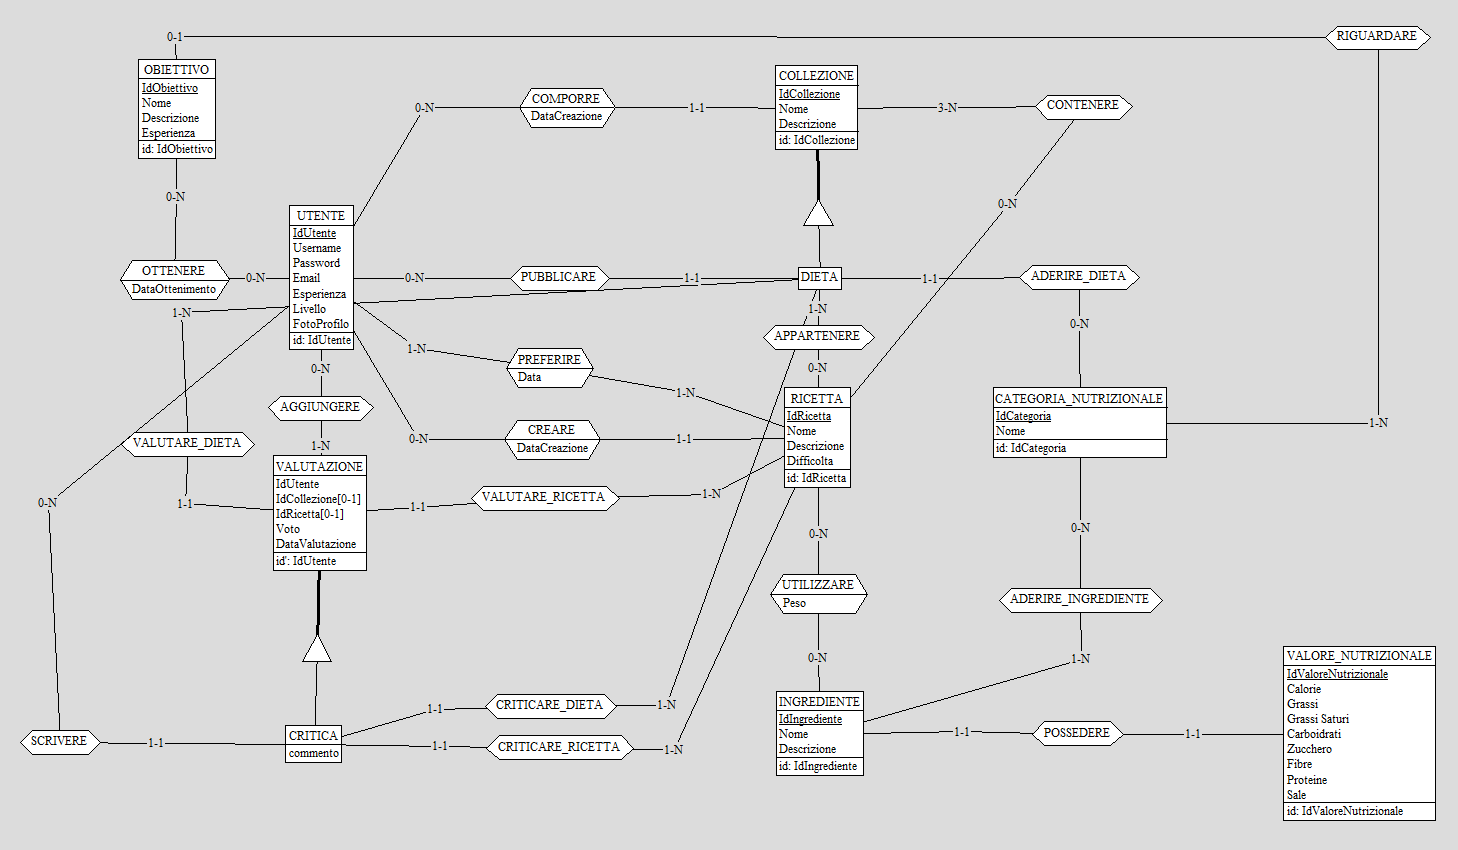
\includegraphics[width=0.9\linewidth]{app_images/schema-concettuale.png}
\end{figure}

\subsection{Valutazione}
Essendo critica una forma avanzata di valutazione
abbiamo optato per una Gerarchia
\begin{figure}[H]
    \centering
    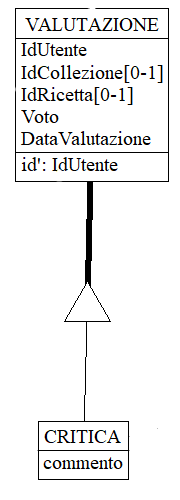
\includegraphics[width=0.2\linewidth]{app_images/valutazione-concettuale.png}
\end{figure}
\subsection{Obiettivo}
La necessità di imporre vincoli all'utente precendentemente espressa
è implementata attraverso l'uso di obiettivi
\begin{figure}[H]
    \centering
    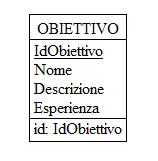
\includegraphics[width=0.45\linewidth]{app_images/obiettivo-concettuale.png}
\end{figure}
\subsection{Categoria}
Un altro limite atto a rendere la ricerca di ricette
piu mirata e le diete piu consistenti e la categoria nutrizionale
che si relaziona con gli ingredienti da cui indirettamente si ricavano le categorie
per una ricetta.
\begin{figure}[H]
    \centering
    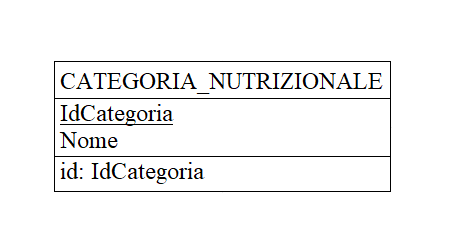
\includegraphics[width=0.6\linewidth]{app_images/categoria-nutrizionale.png}
\end{figure}
\subsection{Collezione}
Molto similmente alle valutazioni, per ottenere una versione limitata
ma libera a tutti gli utenti e una versione di collezione completa( la dieta )
ma non disponibile immediatamente, abbiamo optato per una gerarchia.
\begin{figure}[H]
    \centering
    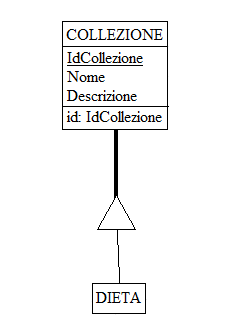
\includegraphics[width=0.6\linewidth]{app_images/collezione-concettuale.png}
\end{figure}
\chapter{Progettazione logica}
capitolo logica
\section{Volume dei dati}
\begingroup
\renewcommand{\arraystretch}{1.5}  % Adjust row padding for this table only
\setlength{\tabcolsep}{10pt}       % Adjust column padding for this table only
\begin{table}[h!]
    \centering   
    \begin{tabular}{|>{\hspace{10pt}}c<{\hspace{10pt}}|>{\hspace{10pt}}c<{\hspace{10pt}}|>{\hspace{10pt}}c<{\hspace{10pt}}|}
        \hline
        Concetto  & Costrutto  & Volume \\
        \hline
        Utente   & Data 2   & Data 3   \\
        Aggungere   & Data 5   & Data 6   \\
        Valutazione   & Data 8   & Data 9   \\
        Ottenere 
        Obiettivo

        \hline
    \end{tabular}  
\end{table}
\endgroup
\begingroup

\section{Operazioni principali e frequenza}
Secondo sottocapitolo
\section{Tabelle degli accessi}
Secondo sottocapitolo
\section{Raffinamento schema}
Secondo sottocapitolo
\section{Analisi rindondanze}
Secondo sottocapitolo
\section{Traduzione di entità e relazioni in associazioni}
Secondo sottocapitolo
\section{Schema relazionale finale}
Secondo sottocapitolo
\section{Traduzione delle operazioni in query SQL}
Secondo sottocapitolo


\chapter{Progettazione applicazione}
\section{Descrizione dell'architettura\\ dell'applicazione realizzata}
Abbiamo sviluppato un'applicazione Social Media di ricette culinarie per dispositivi mobile in linguaggio C\# utilizzando il framework .NET MAUI (utilizzato per la creazione di applicazioni mobile).
Per le connesioni al database viene utilizzata la libreria C\# MySQLConnector e il database risiede in un server MySQL.
Per ogni tabella contenuta nel DB viene creata una corrispettiva classe che la rappresenta all'interno del
model dell'applicazione. Inoltre abbiamo creato una classe DBService che gestisce le connessioni effettuate al database e presenta vari metodi:
\begin{itemize}
    \item TryConnection(DBCredentials dbc): prende in input le credenziali per accedere al database e restituisce un booleano sul risultato della connessione al database.
    \item ExistInTable(string query): restituisce un booleano in base al numero di elementi che produce la query data (0 elementi prodotti = false)
    \item GetData(string query): restituisce una lista di elementi generici in base alla tabella su cui viene effettuata la query e al tipo specificato.
    \item InsertElement(List〈Tuple〈string, object〉〉 values, string query): inserisce gli elementi nella tabella specificata nella query inserendo nei valori della query non settati (?) il rispettivo valore contenuto nella lista di tuple.
    \item RemoveOrUpdateElement(string query): rimuove o aggiorna la riga di una tabella seguendo la query data.
\end{itemize}
All'avvio dell'applicazione, se si tratta del primo avvio, comparirà la schermata di Login e Registrazione.
\begin{figure}[h!]
    \begin{minipage}{.5\textwidth}
        \centering
        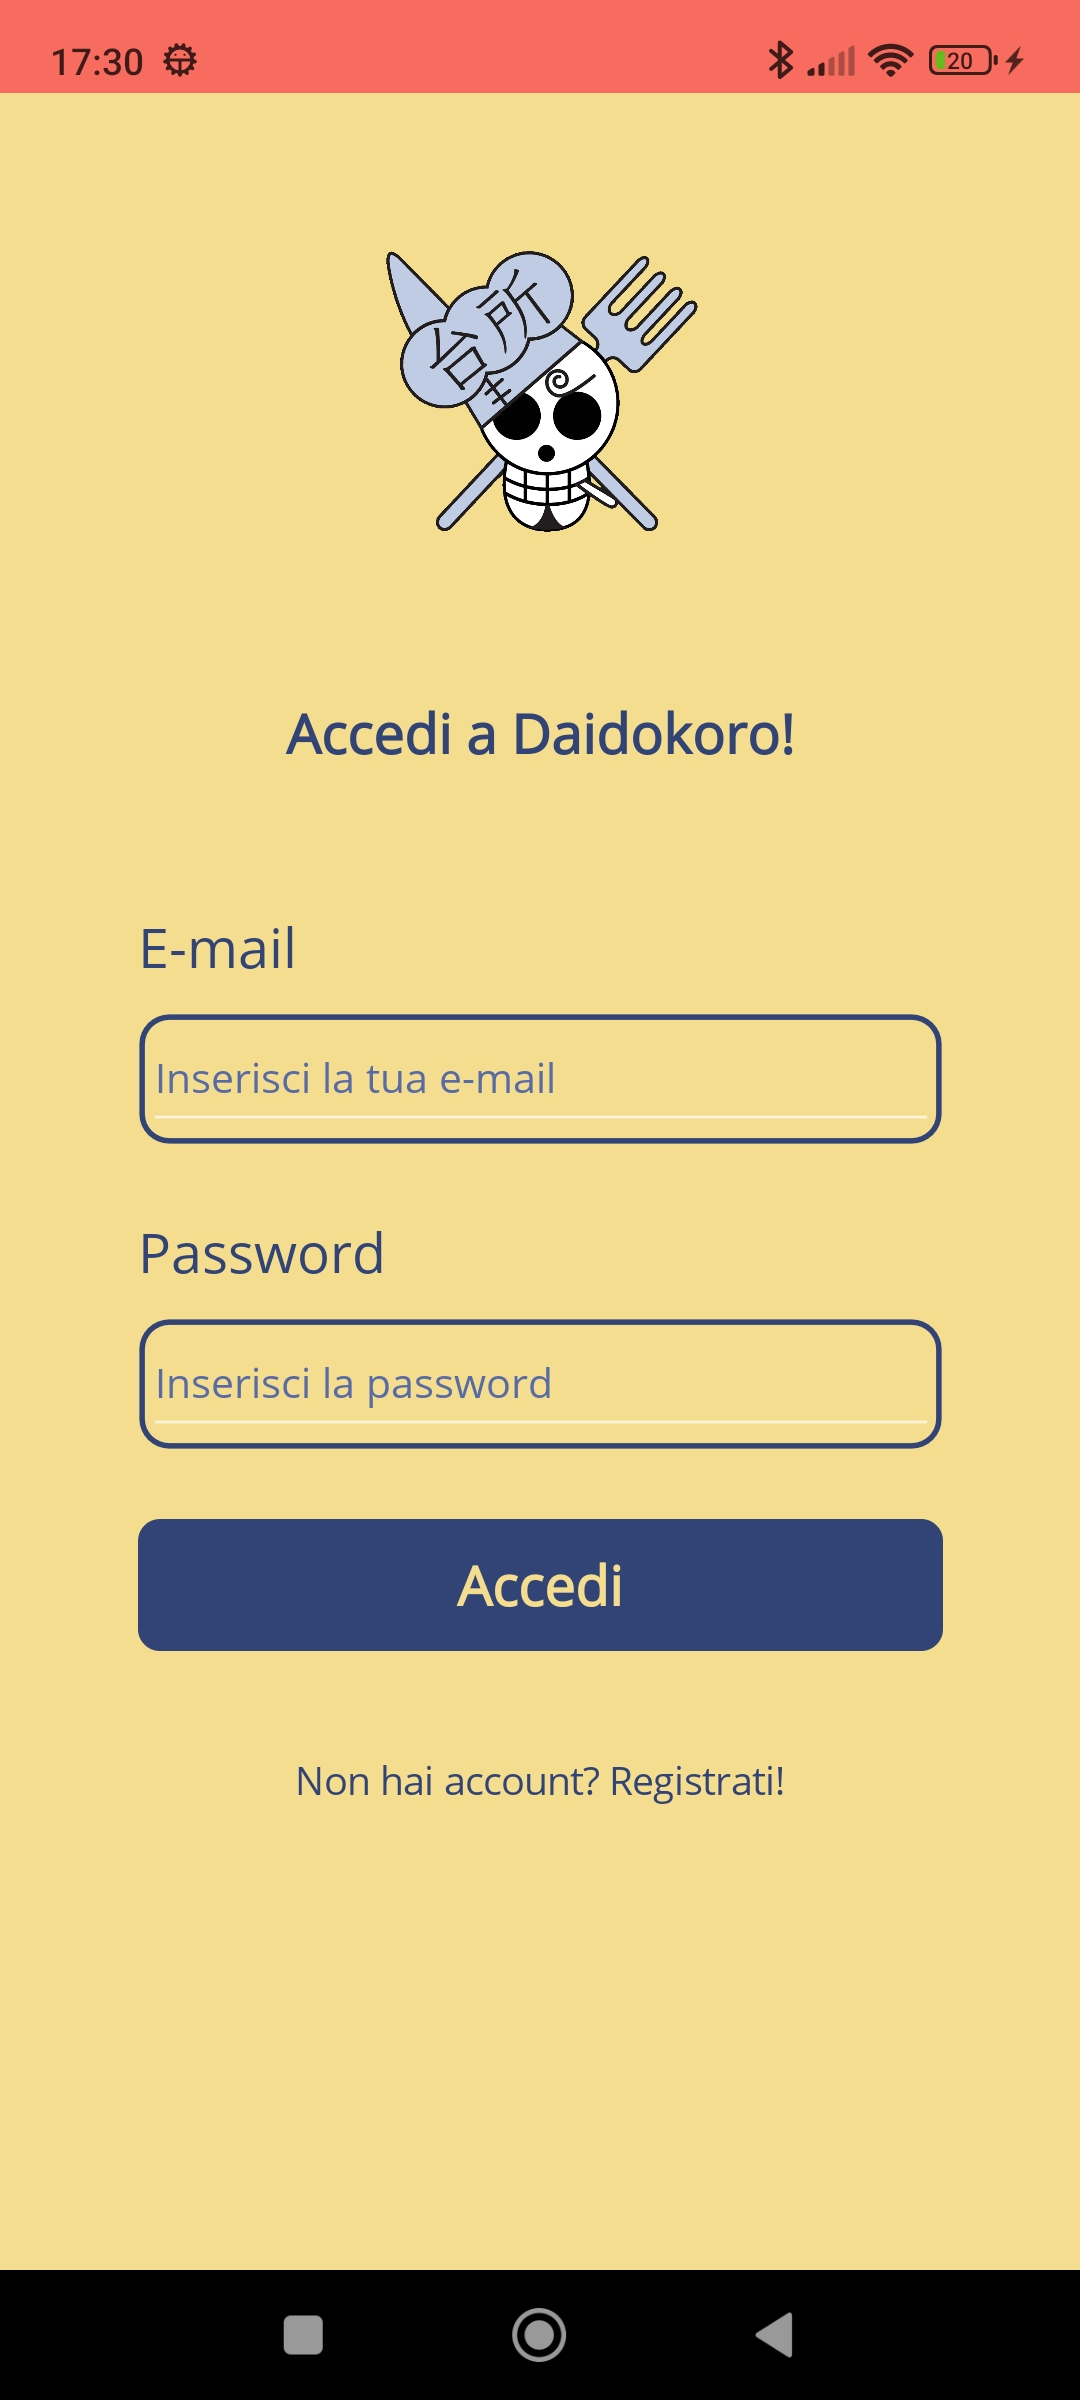
\includegraphics[width=0.9\linewidth]{app_images/Login.jpg}
    \end{minipage}
    \begin{minipage}{.5\textwidth}
        \centering
        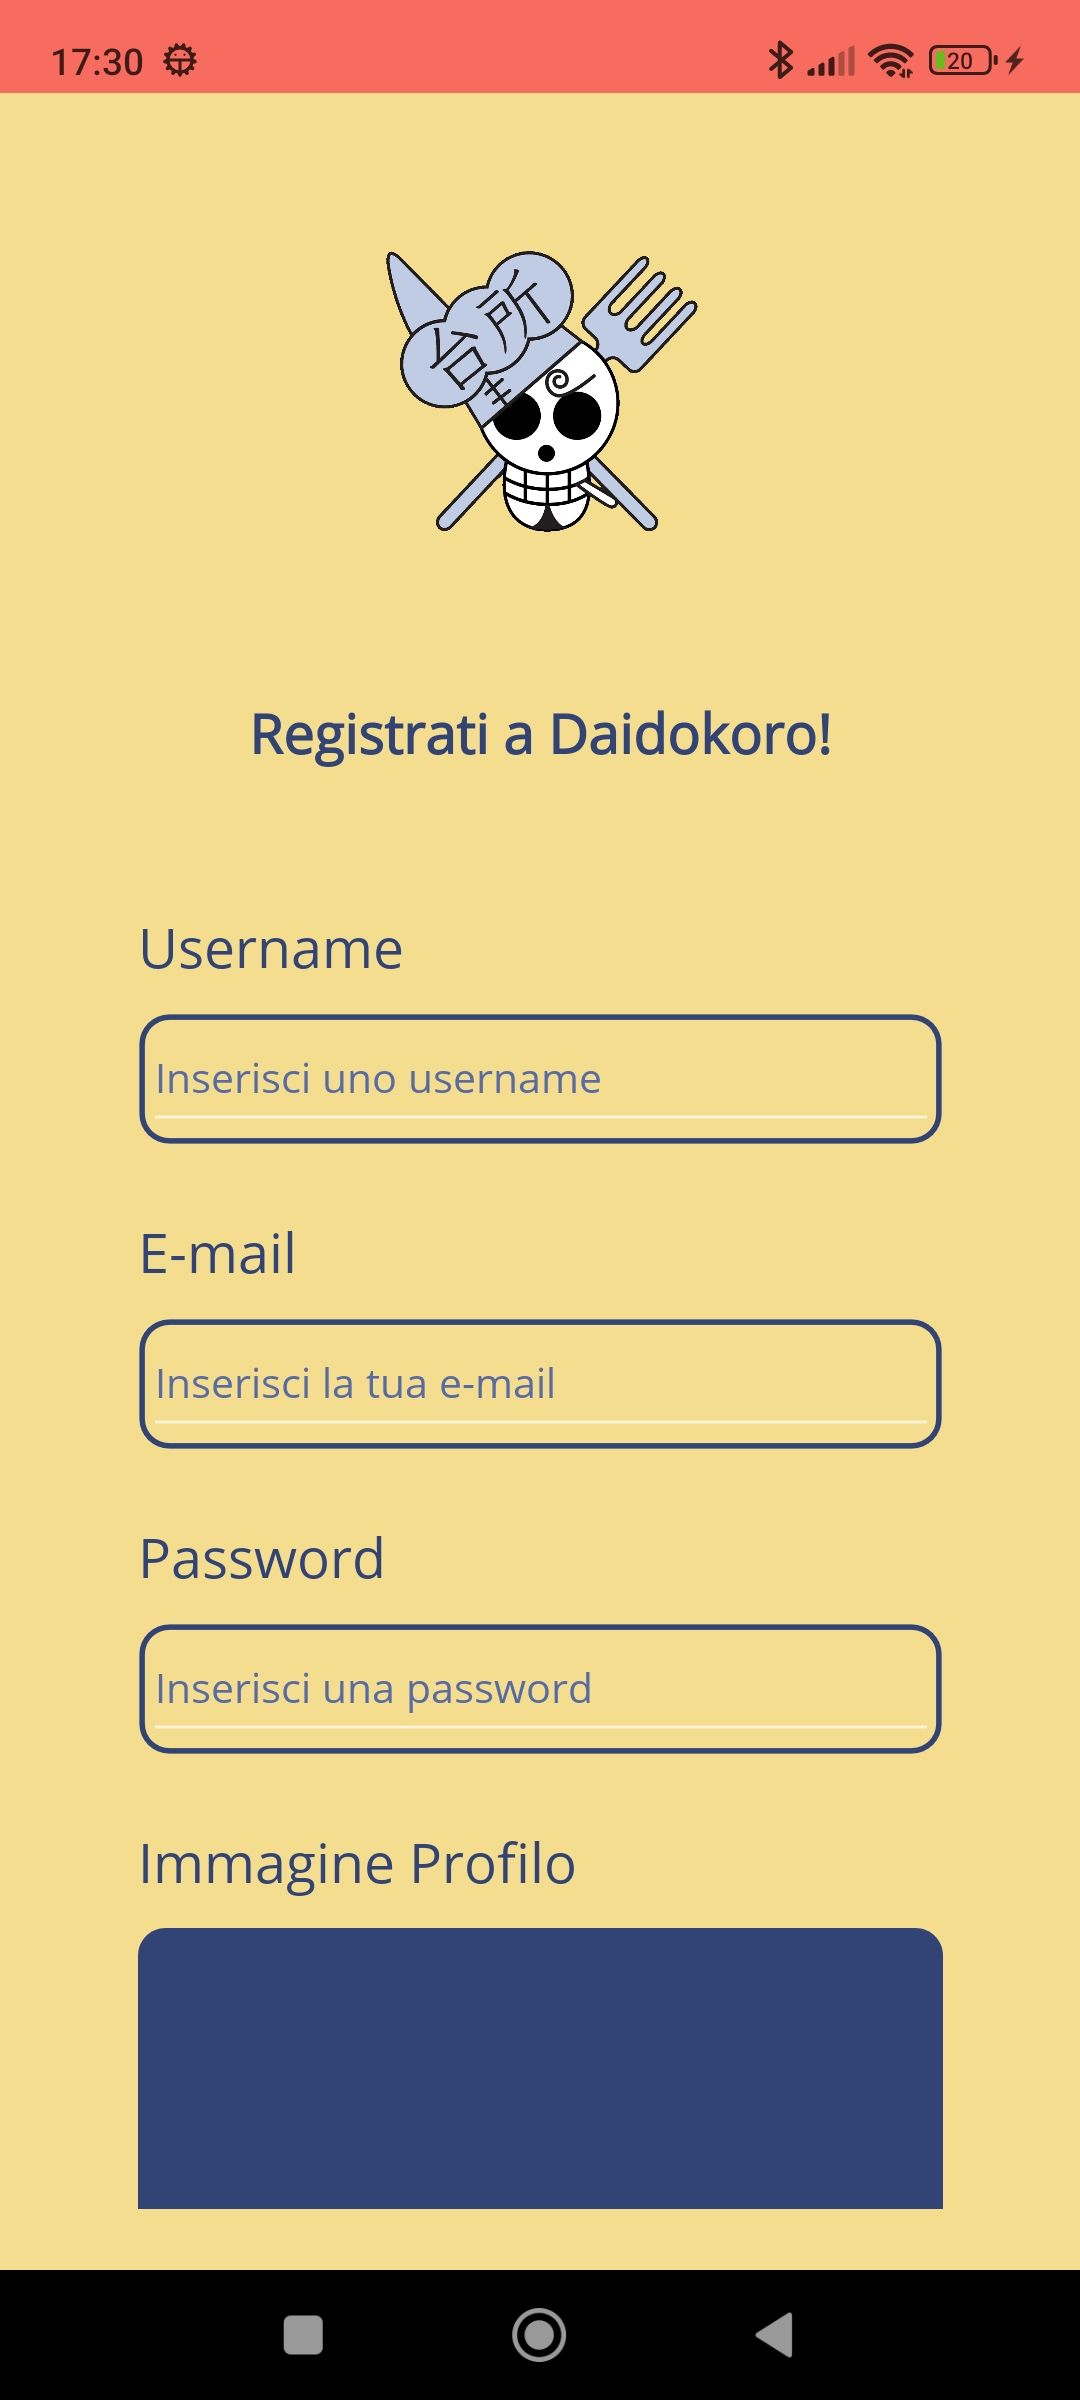
\includegraphics[width=0.9\linewidth]{app_images/Register.jpg}
    \end{minipage}
\end{figure}
\\Dopo essersi registrati e aver effettuato l'accesso verrà memorizzato nei dati dell'applicazione installata l'identificativo dell'utente che ha effettuato l'accesso in modo da poter reindirizzare l'utente sulla schermata principale ad ogni avvio successivo dell'app e caricare i suoi dati.
\\\\\\\\\\\\\\Nella Home Page è possibile visualizzare le 3 ricette con più like.
\\Clickando, invece, sull'icona centrale del menu di navigazione sovrastante, si potrà andare sulla pagina di navigazione delle ricette, collezioni e diete
\begin{figure}[h!]
    \begin{minipage}{.5\textwidth}
        \centering
        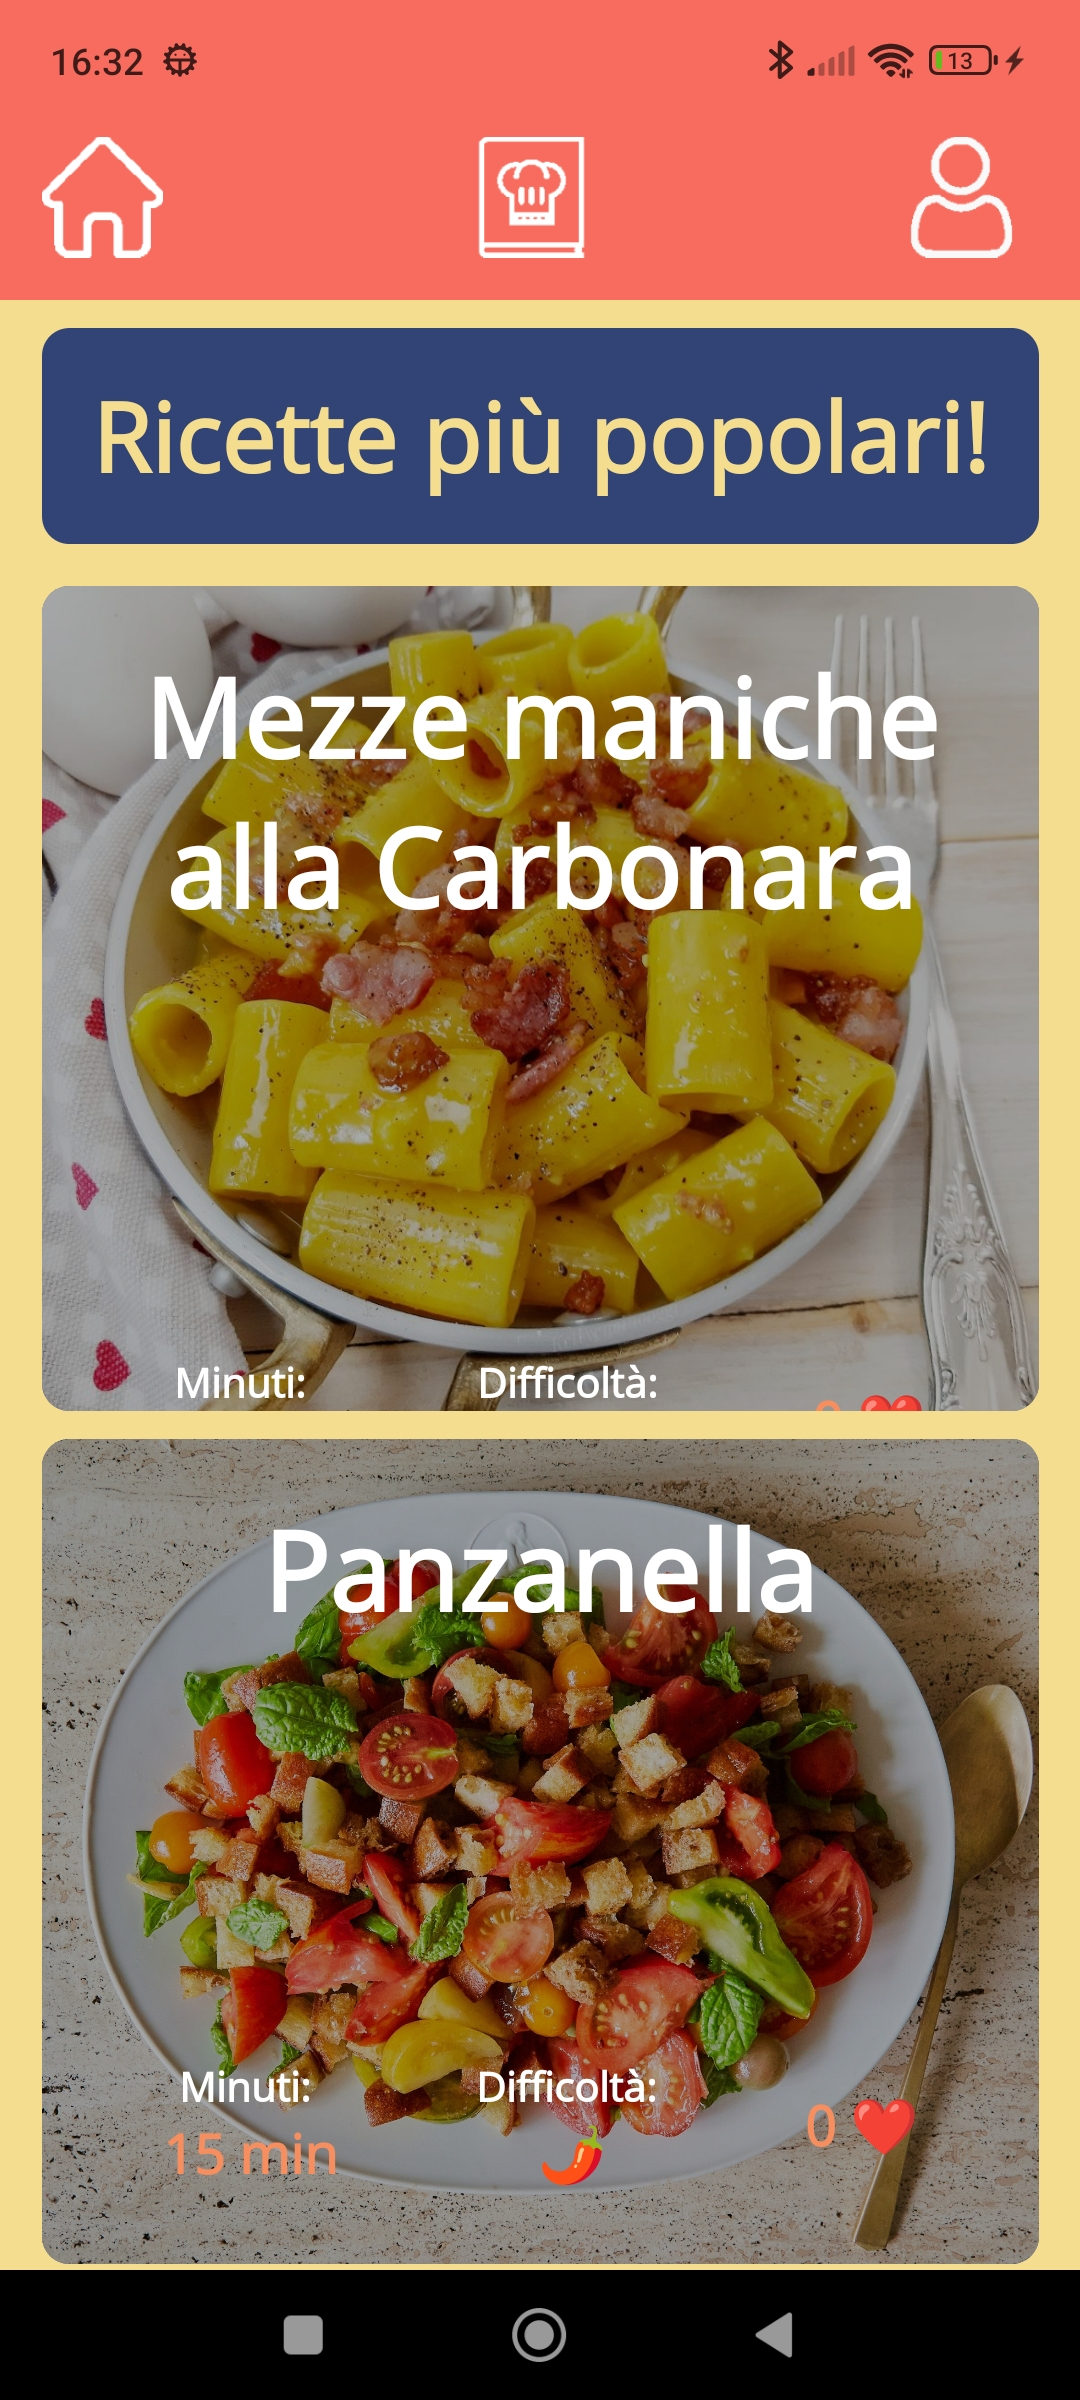
\includegraphics[width=0.9\linewidth]{app_images/HomePage.jpg}
    \end{minipage}
    \begin{minipage}{.5\textwidth}
        \centering
        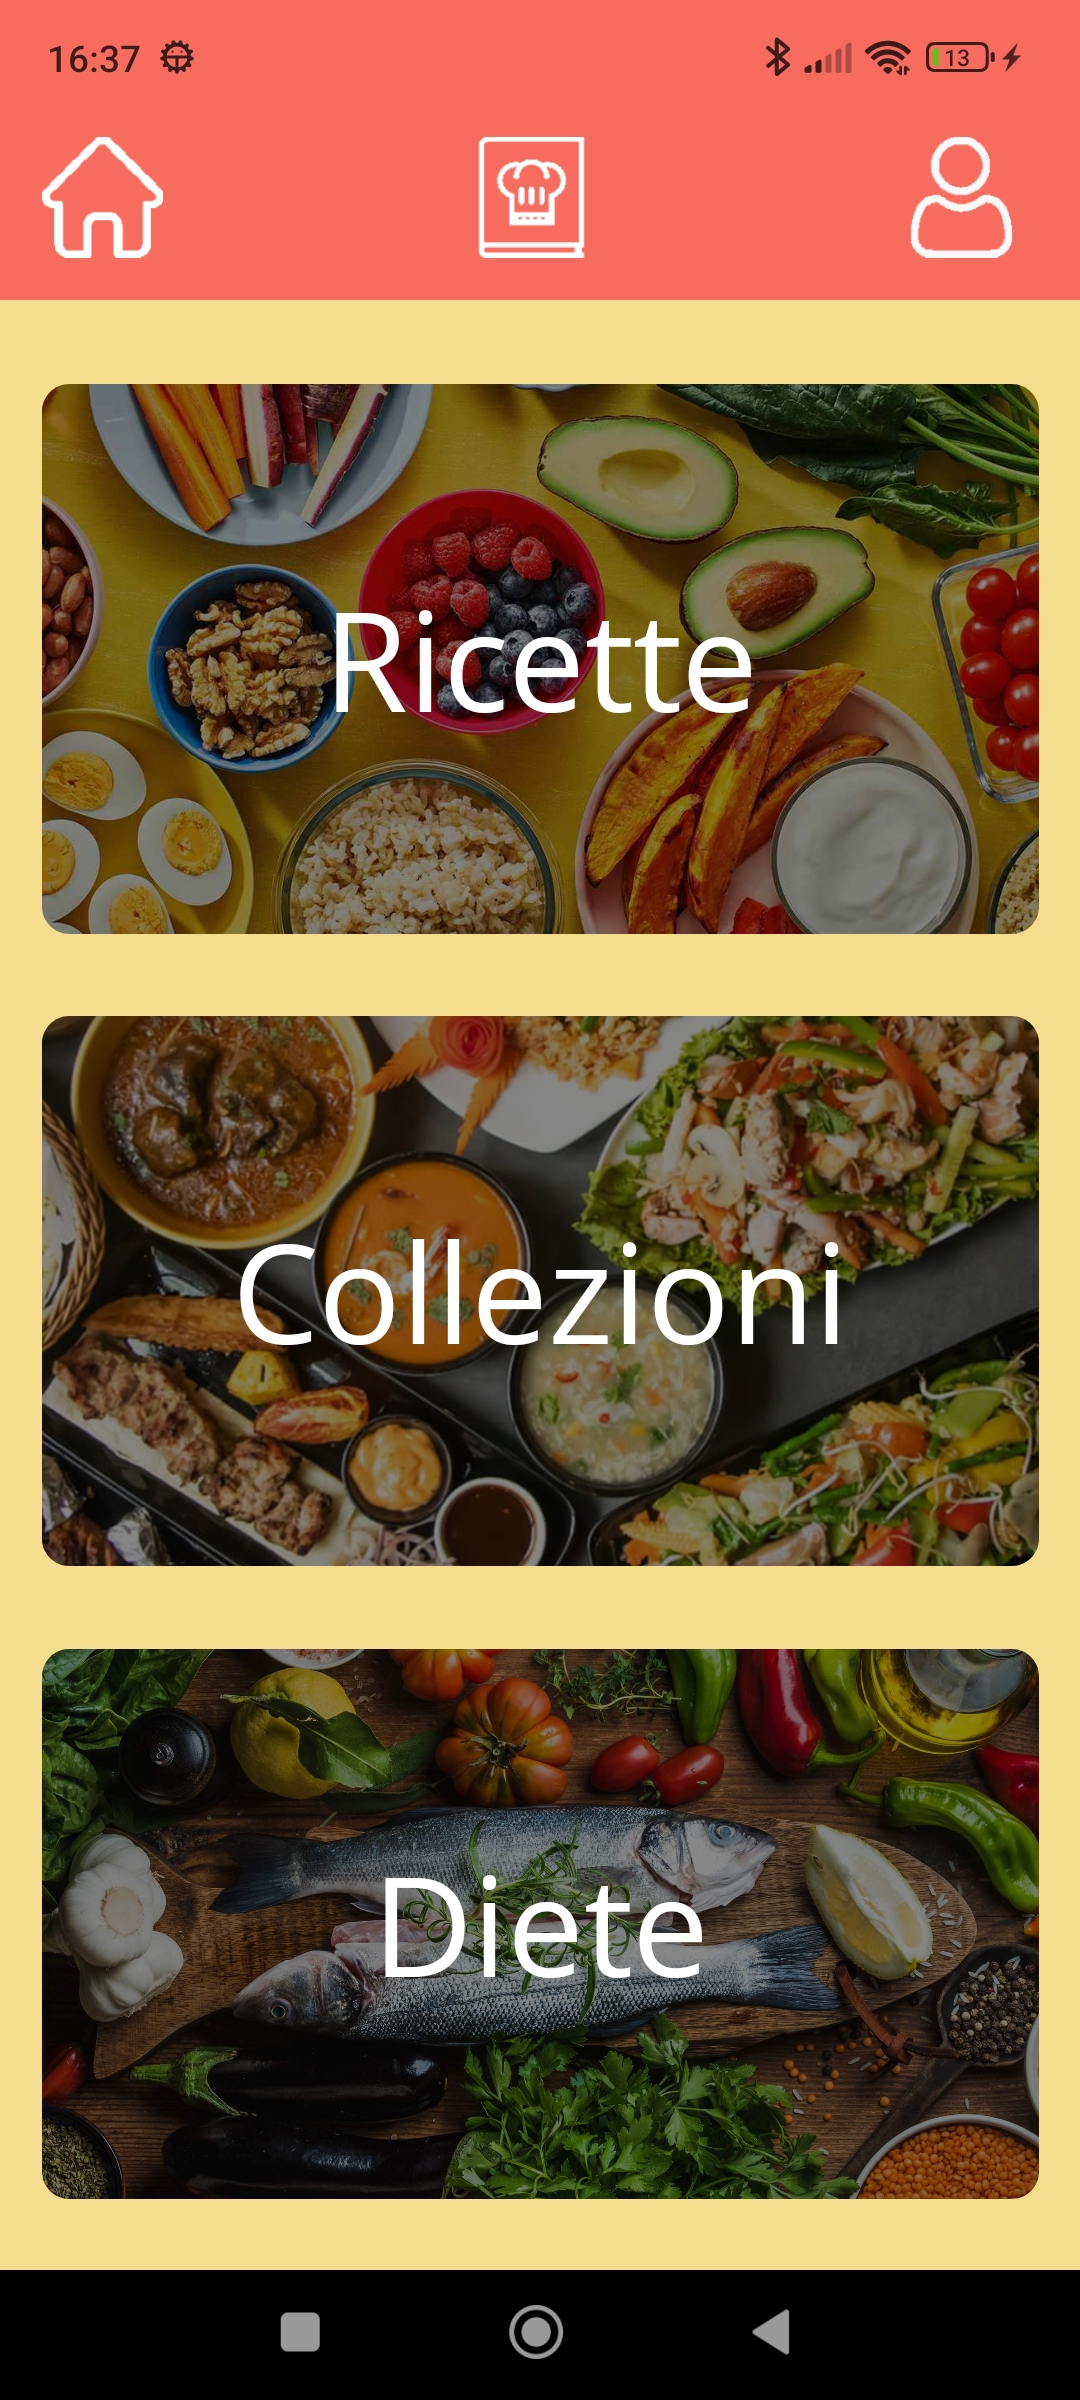
\includegraphics[width=0.9\linewidth]{app_images/BrowsePage.jpg}
    \end{minipage}
\end{figure}
\\Successivamente nella pagina di navigazione in base all'elemento clickato comparirà la pagina di visualizzazione della lista del rispetto elemento.
\\\\\\\\Di seguito si ha a sinistra la pagina con la lista delle ricette di qualunque utente con la rispettiva barra di ricerca e filtri.
Mentre a destra la pagina con la lista di collezioni di qualunque utente e la barra di ricerca.
\begin{figure}[h!]
    \begin{minipage}{.5\textwidth}
        \centering
        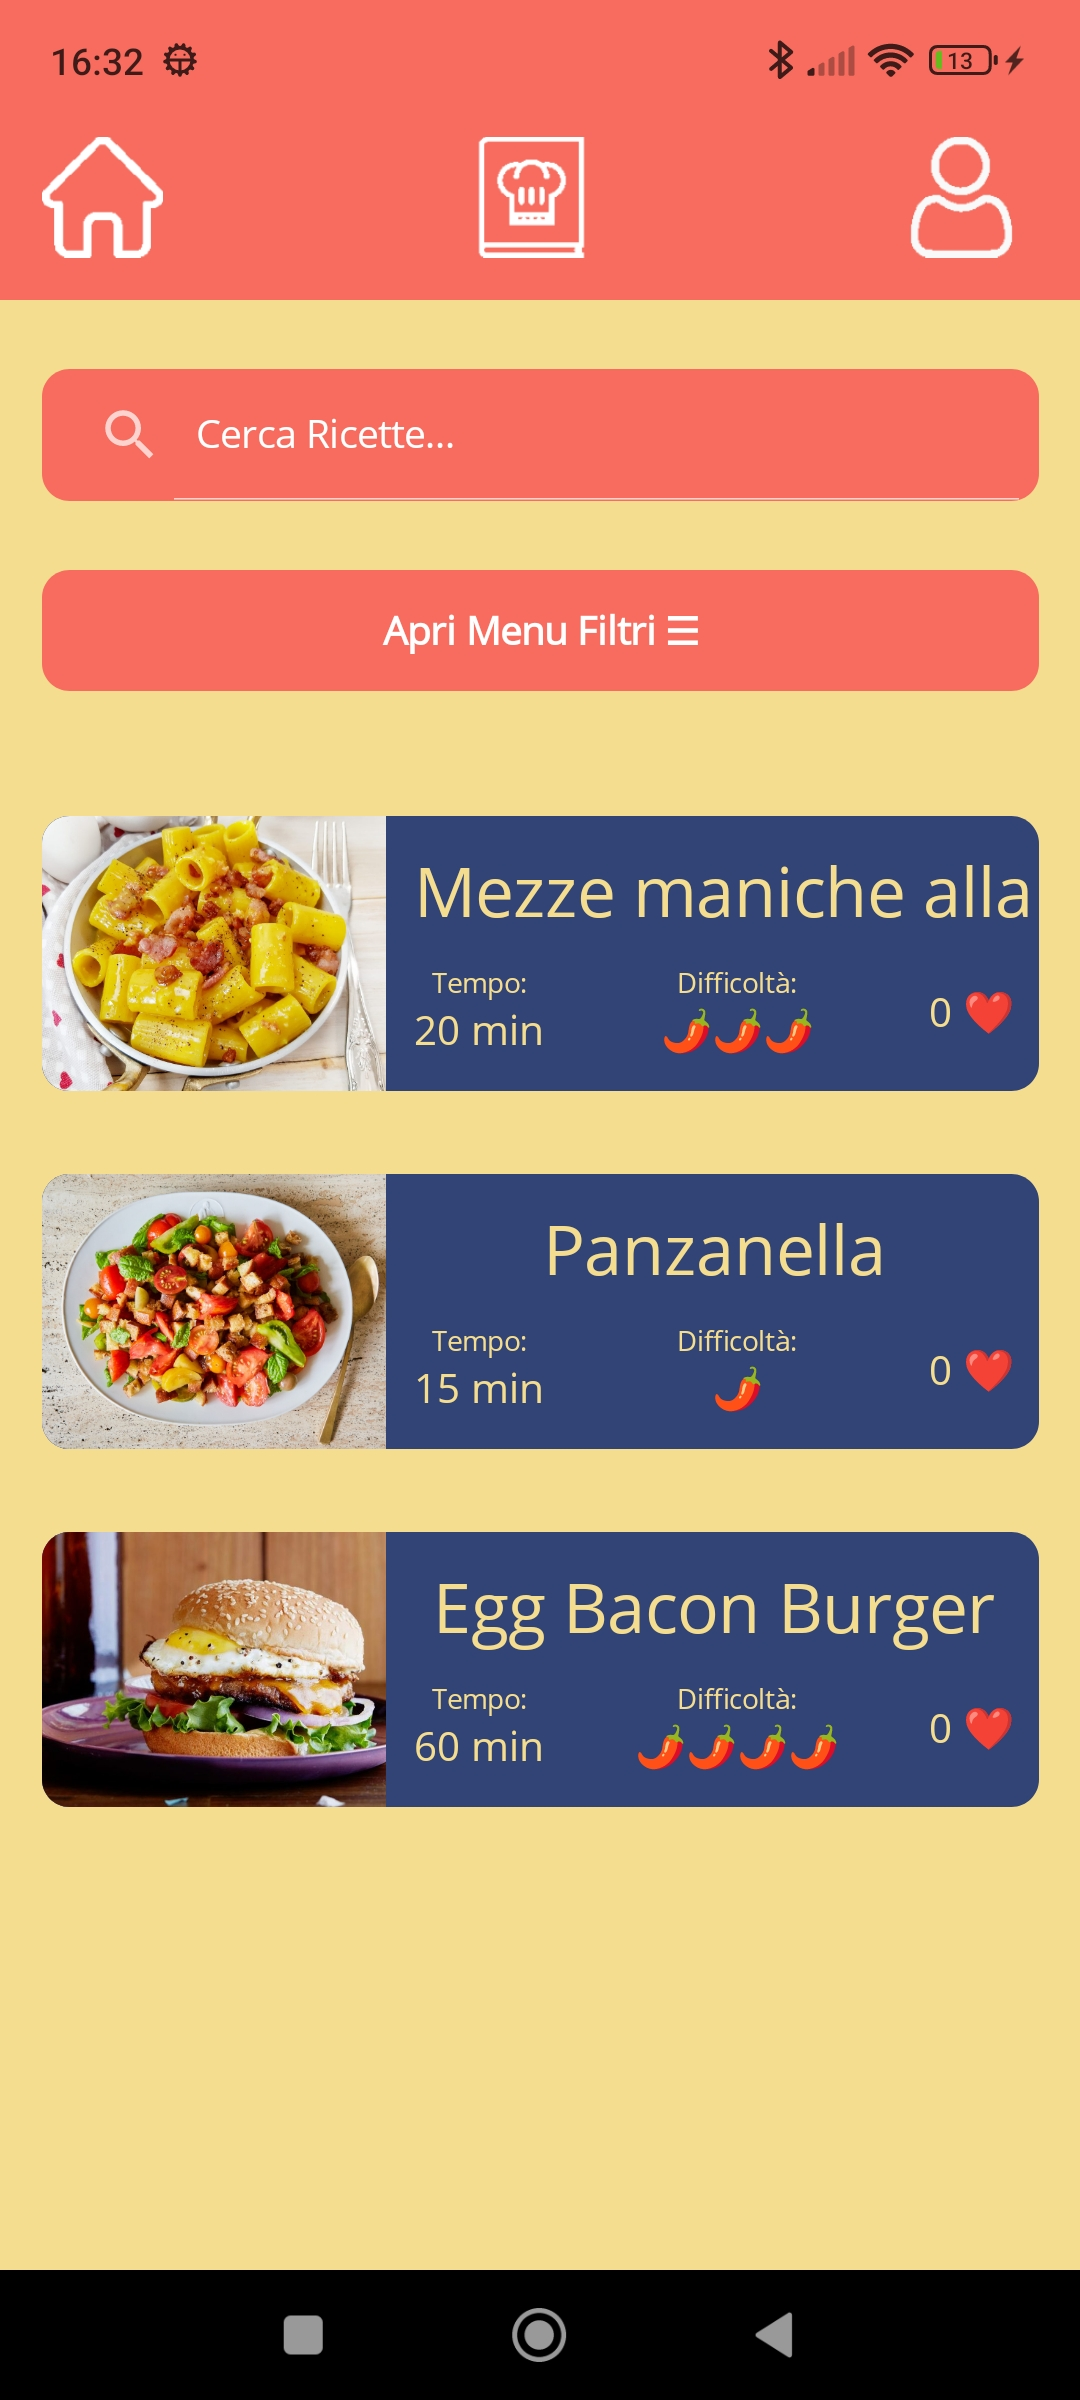
\includegraphics[width=0.9\linewidth]{app_images/RecipeList.jpg}
    \end{minipage}
    \begin{minipage}{.5\textwidth}
        \centering
        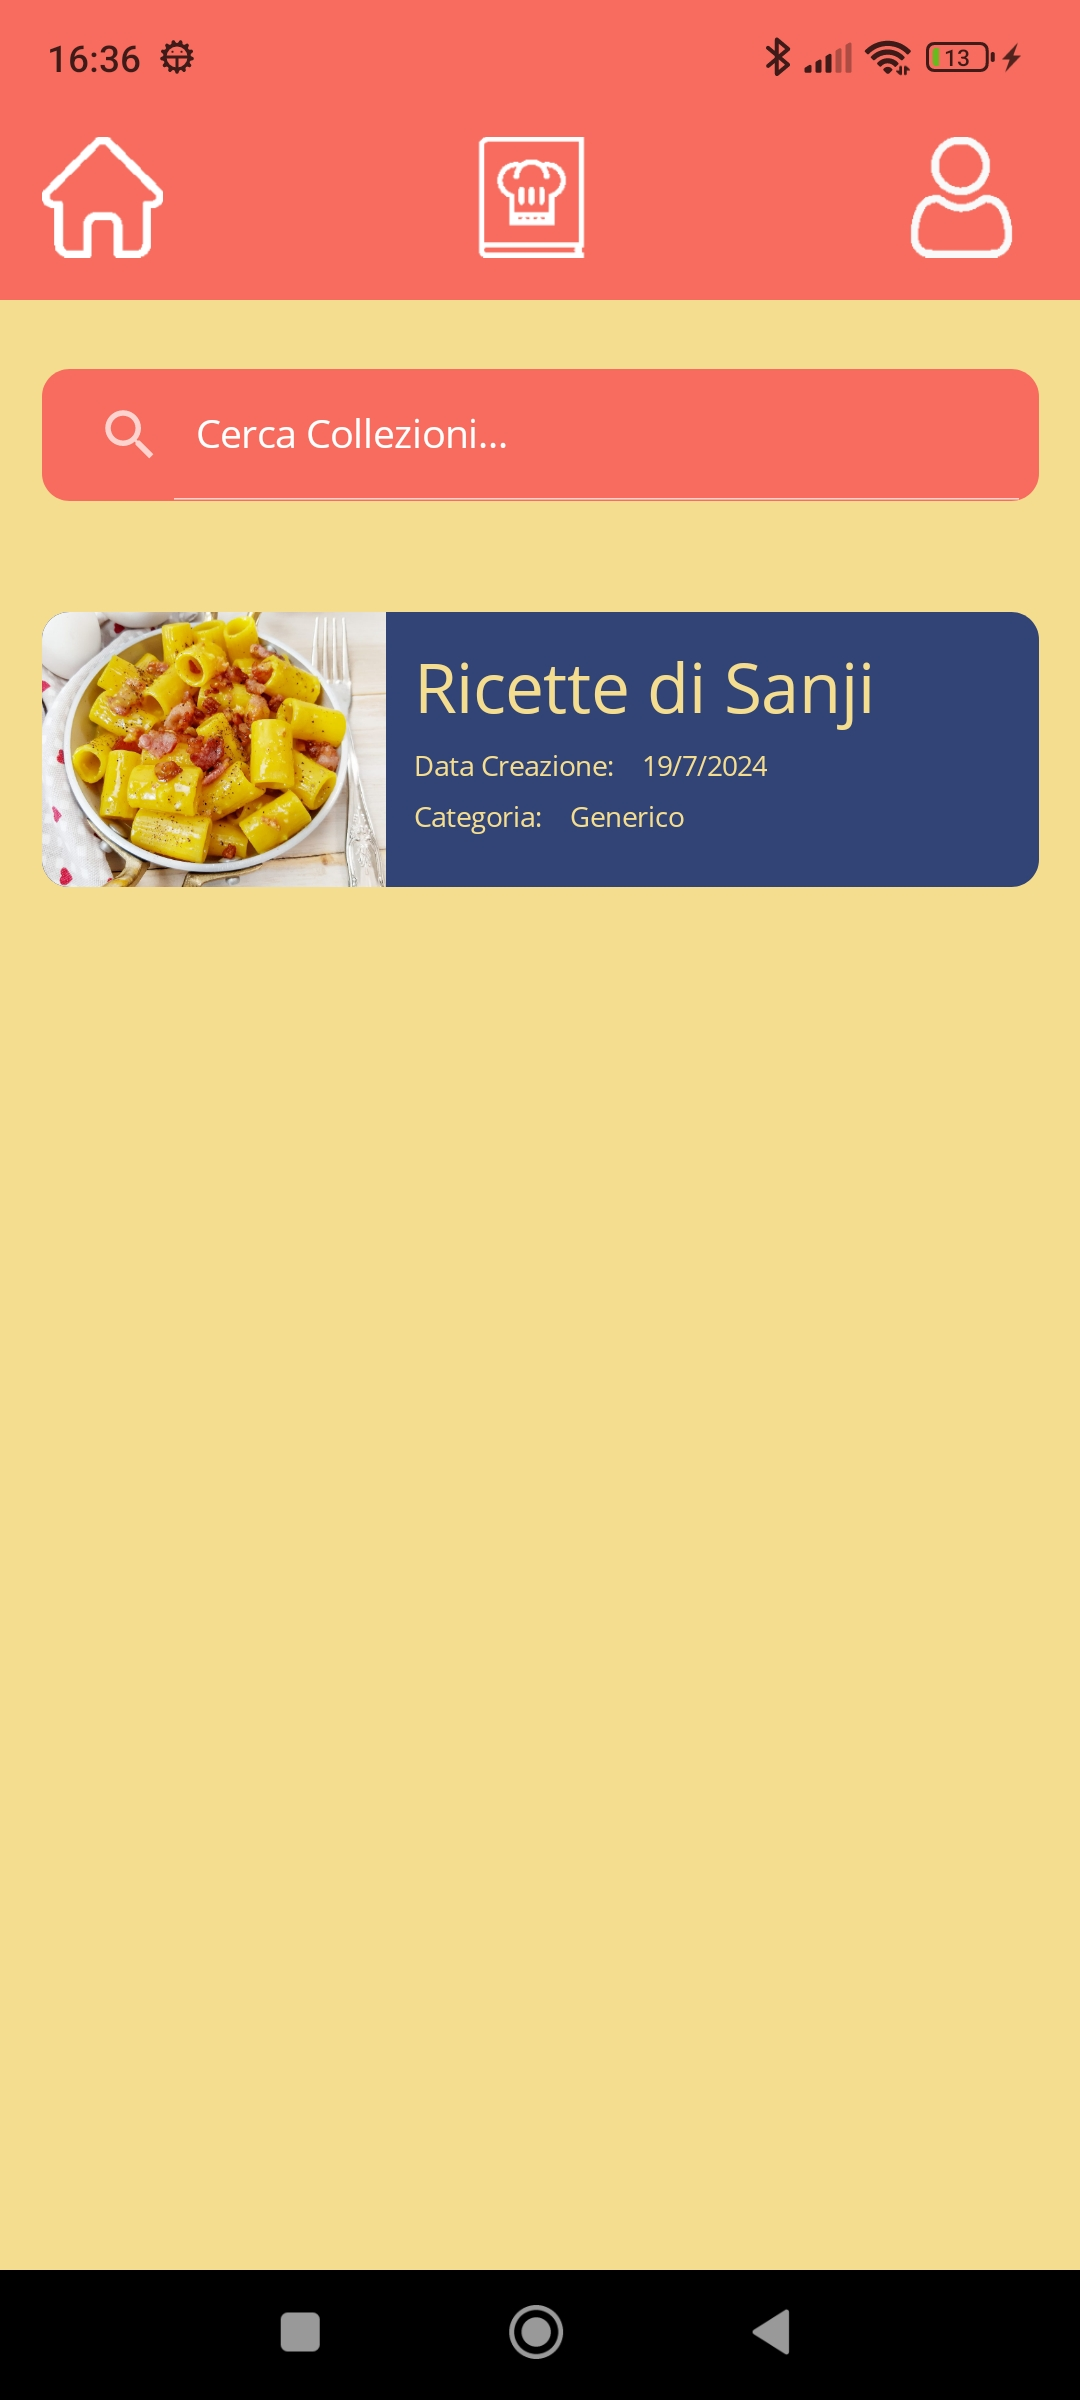
\includegraphics[width=0.9\linewidth]{app_images/CollectionList.jpg}
    \end{minipage}
\end{figure}
\\\\Ogni ricetta nella lista presenta l'immagine, il nome, il tempo di preparazione, difficoltà rappresentata da 1 a 5 con l'emoji di un peperoncino e il numero di like ricevuti da utenti.
Mentre le collezioni avranno come immagine quella della ricetta con più like nella collezione, la data di creazione e la categoria.
\\\\La pagina delle diete è composta come quella delle collezioni ma presente un menu dei filtri come quello delle ricette oltre alla barra di ricerca.
\begin{figure}[h!]
    \begin{minipage}{.5\textwidth}
        \centering
        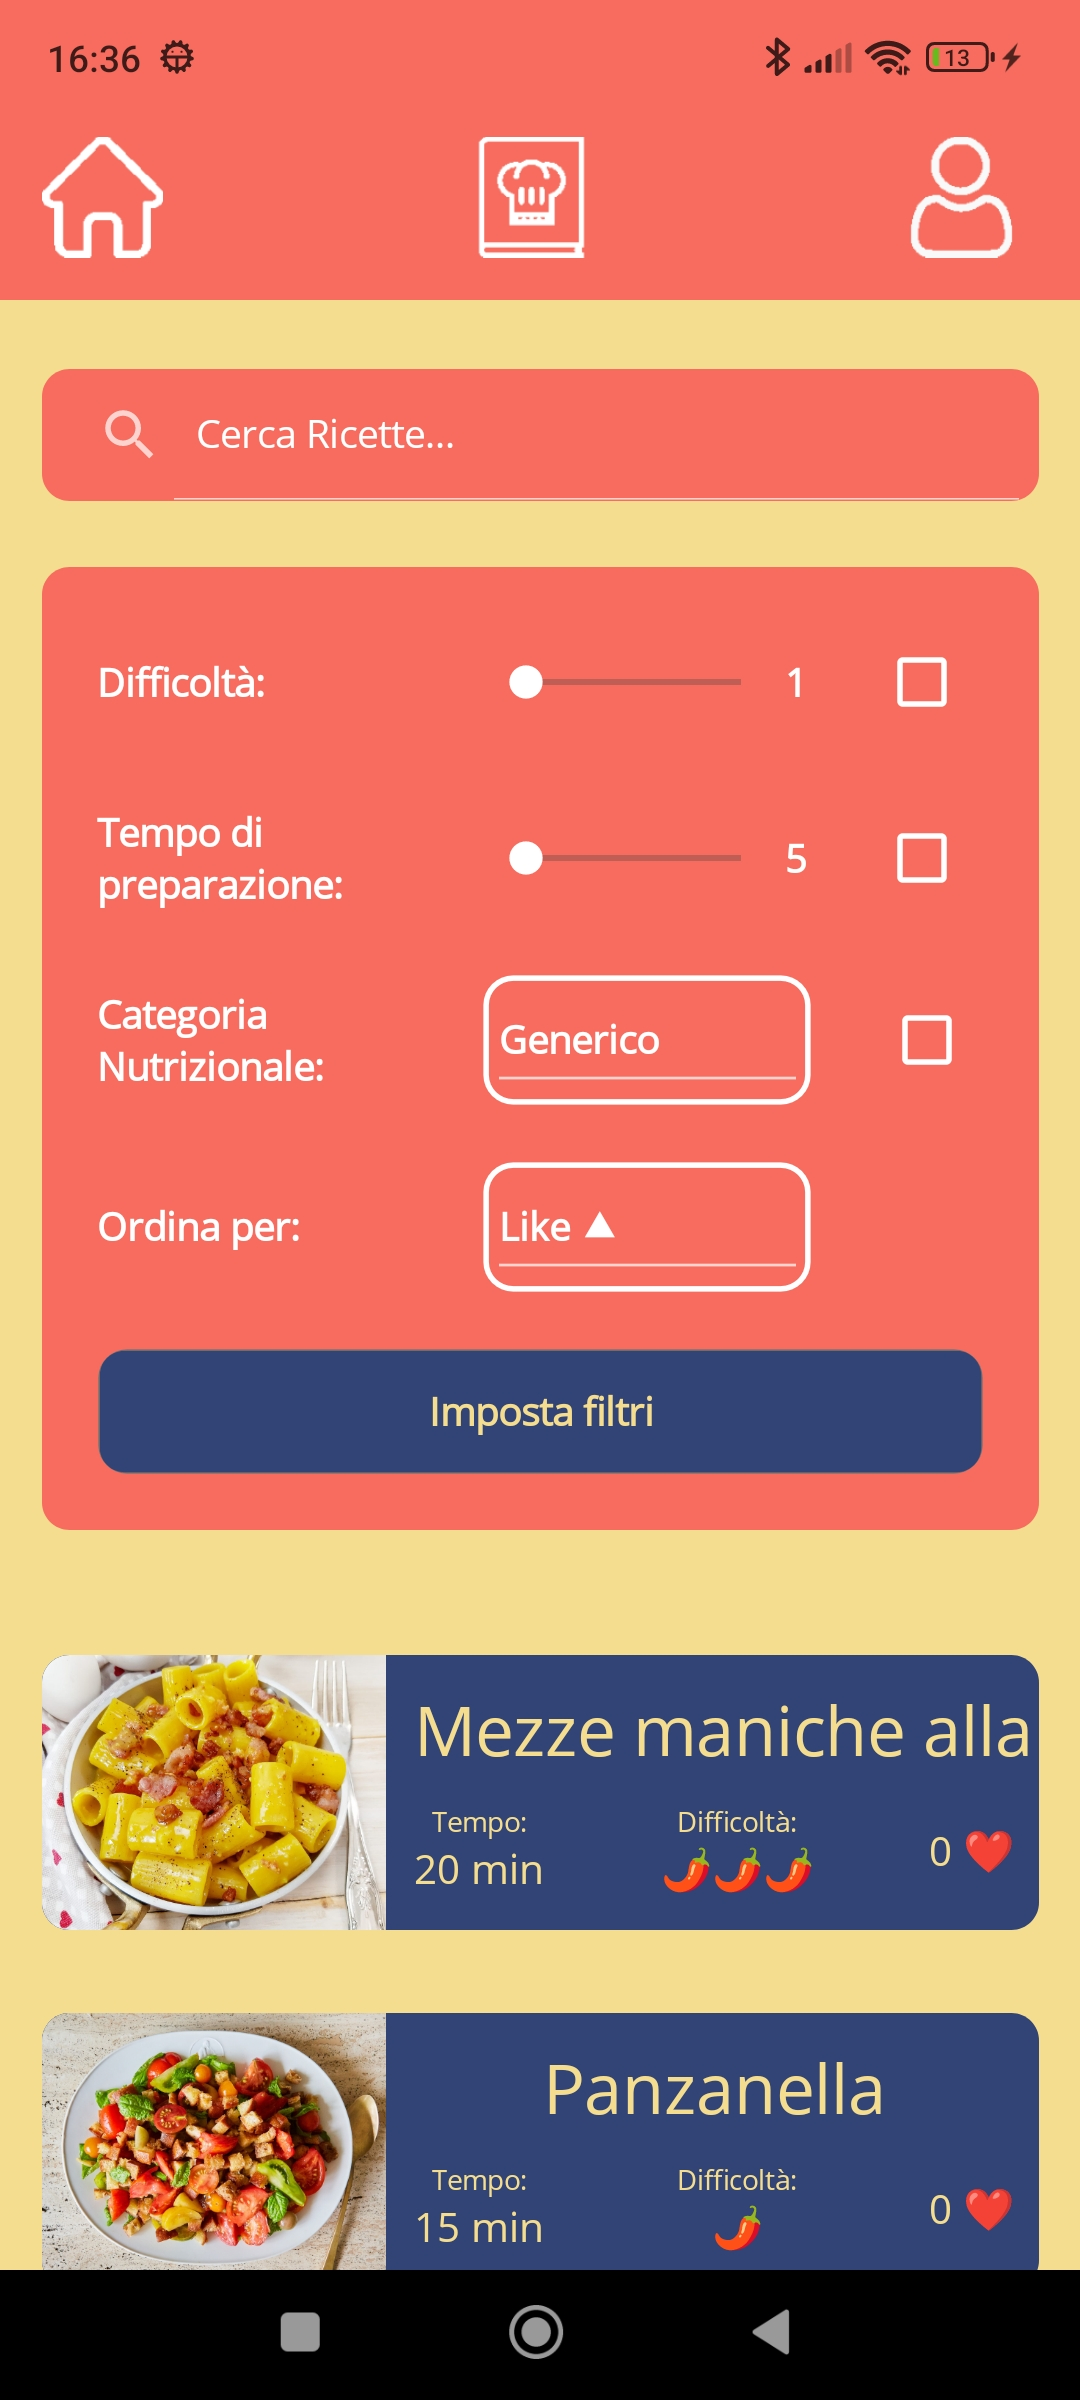
\includegraphics[width=0.9\linewidth]{app_images/Filter.jpg}
    \end{minipage}
    \begin{minipage}{.5\textwidth}
        \centering
        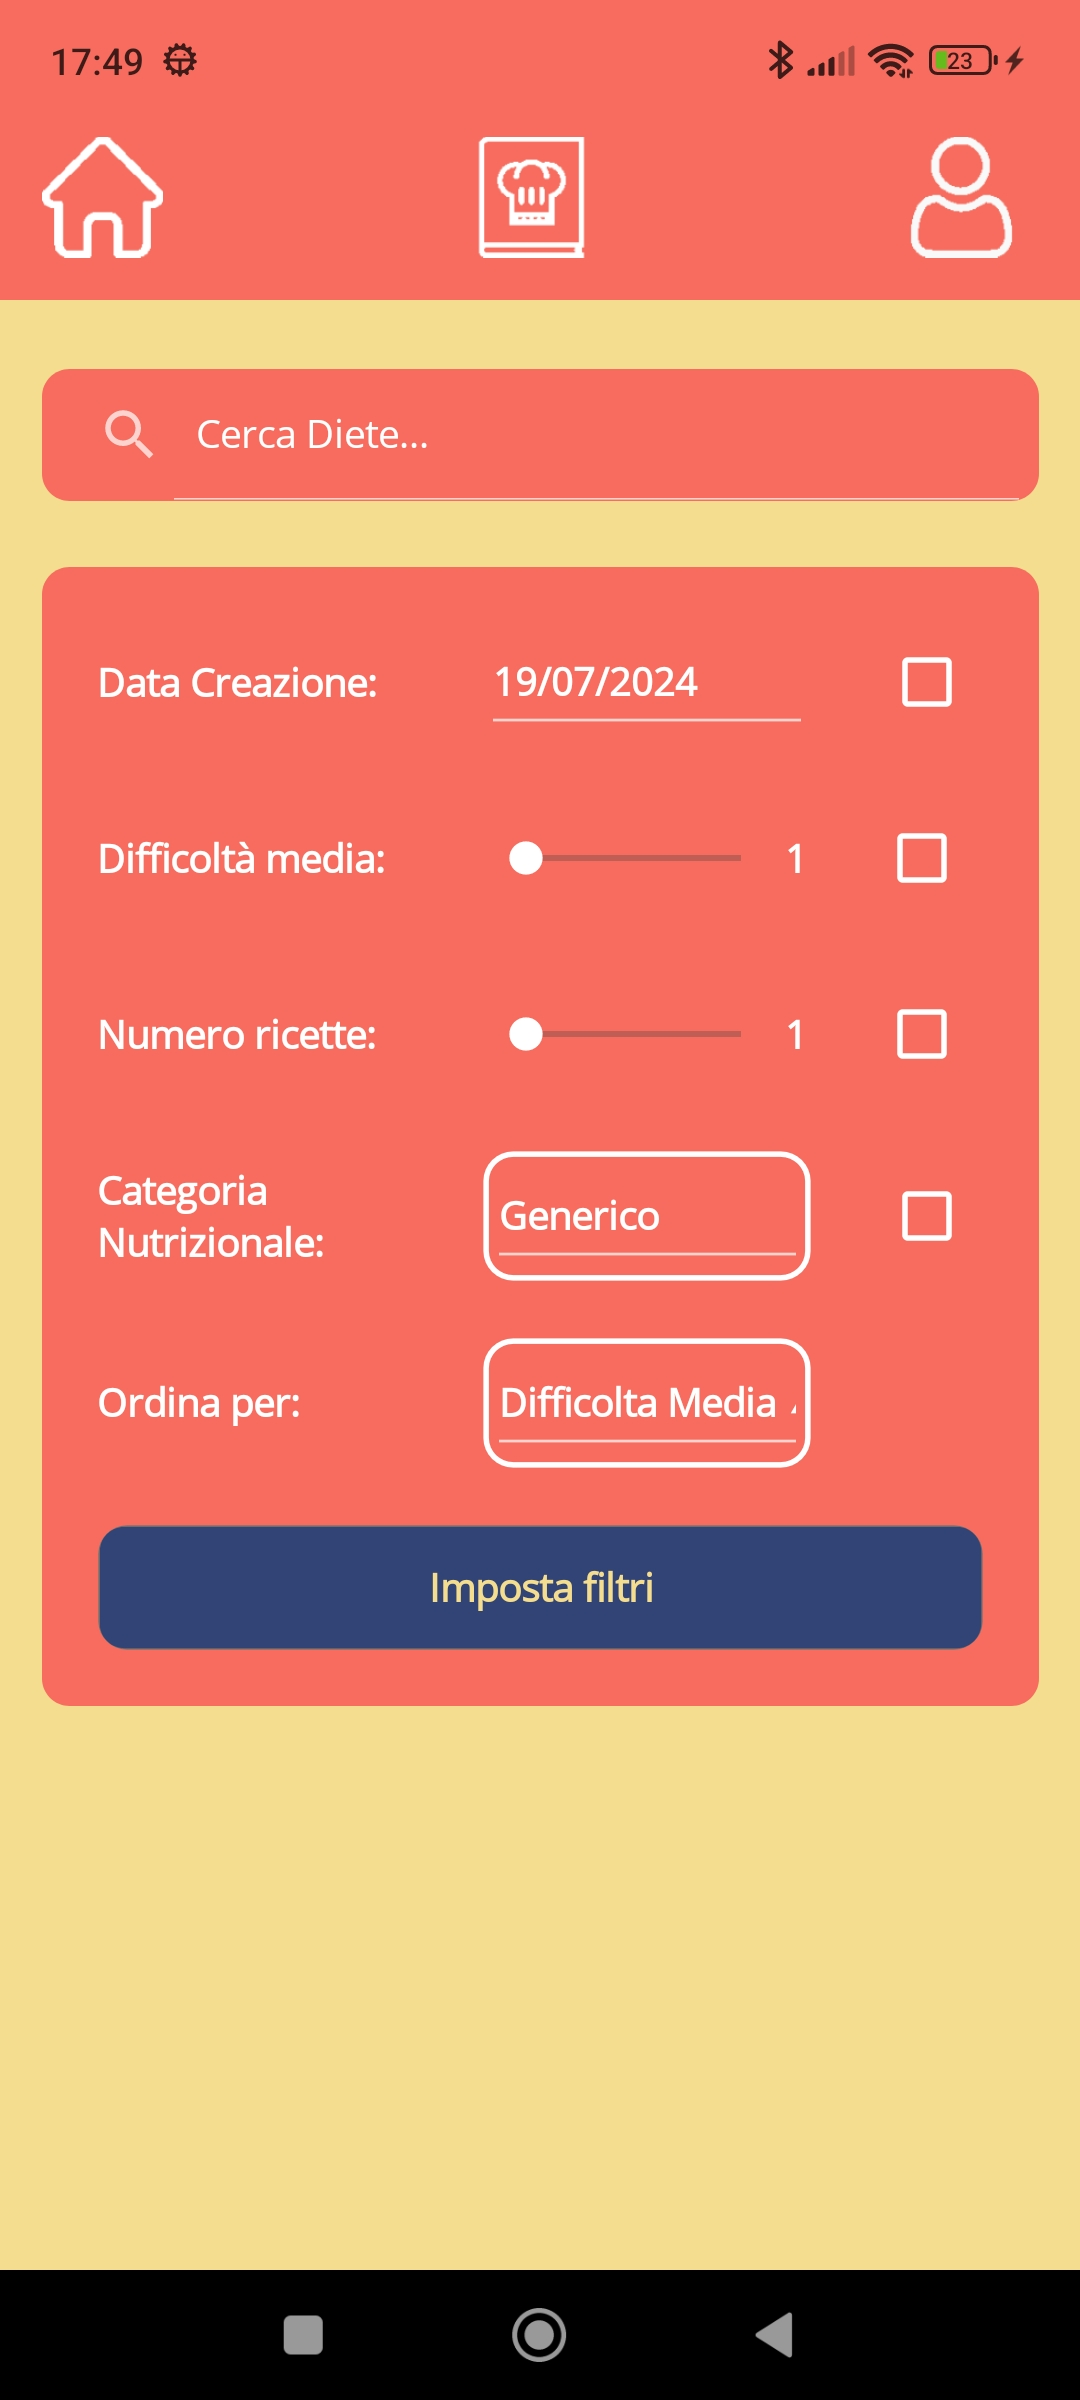
\includegraphics[width=0.9\linewidth]{app_images/Filter2.jpg}
    \end{minipage}
\end{figure}
\\La barra di ricerca delle diete effettuerà la ricerca di una ricetta in base al nome, al nome degli ingredienti associati e al nome della categoria nutrizionale degli ingredienti, mentre quella delle collezioni e delle diete cercherà in base al nome della collezione/dieta e al nome delle ricette contenute.
\\\\Per quanto riguarda le ricette, il menu dei filtri contiene uno slider per la difficoltà e uno per il tempo di preparazione, un selettore per la categoria nutrizionale e un selettore per l'ordinamento da effettuare sulle ricette filtrate.
Mentre il menu dei filtri delle diete contiene un selettore per la data di creazione, uno slider per la difficoltà media delle ricette contenute nella dieta, uno slider per il numero massimo di ricette nella dieta e i due selettori per la categoria nutrizionale della dieta e l'ordinamento sulle diete filtrate.
\\\\\\\\\\Quando si va su una delle pagine contenenti le liste di elementi, clickando su un elemento si andrà alla pagina del singolo elemento con tutte le informazioni specifiche. 
Di seguito si ha la pagina di una ricetta.
\begin{figure}[h!]
    \begin{minipage}{.5\textwidth}
        \centering
        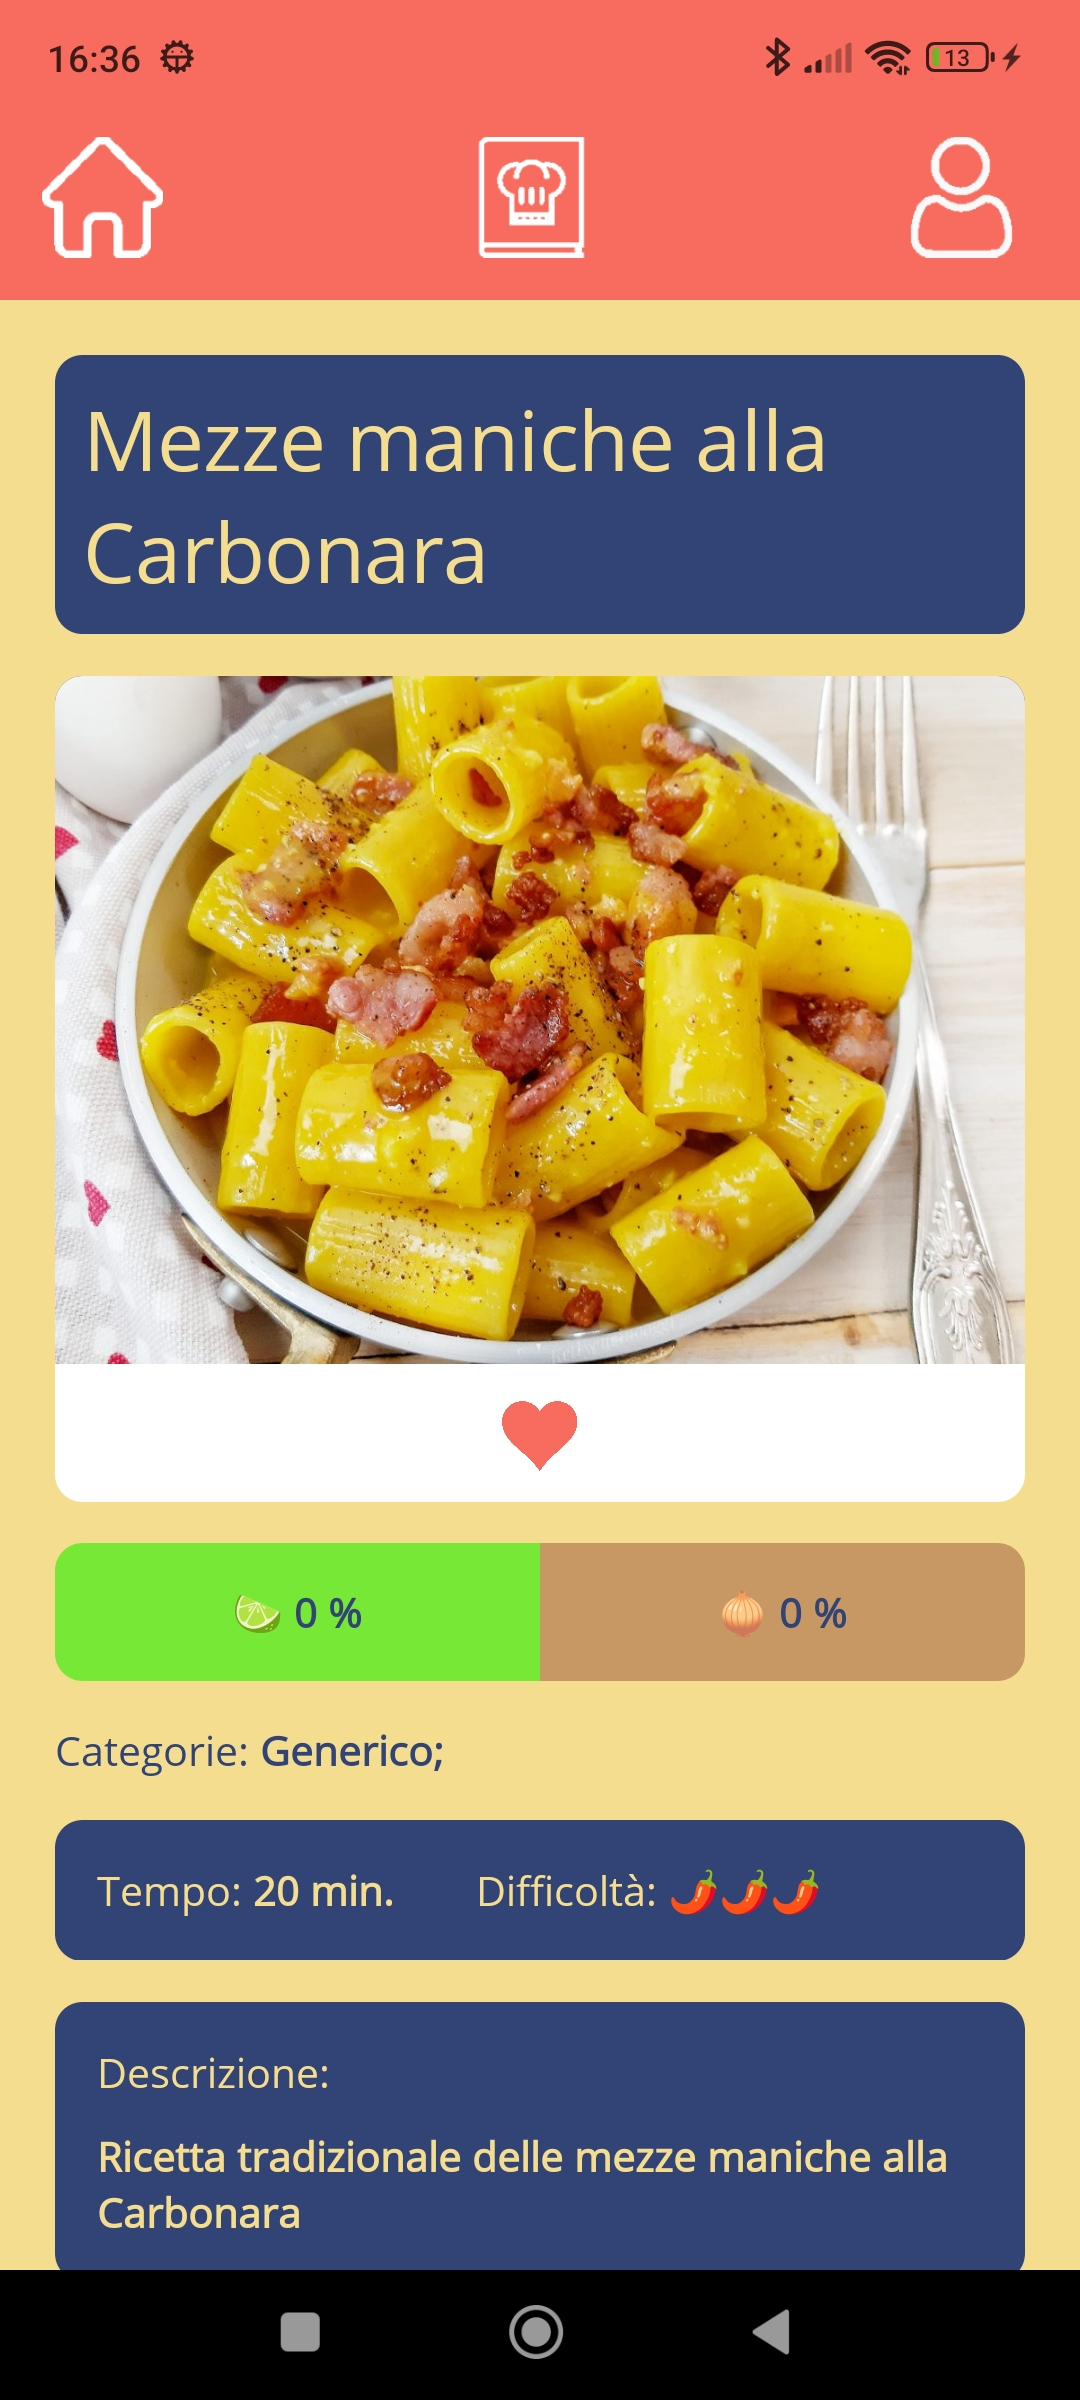
\includegraphics[width=0.9\linewidth]{app_images/Liked.jpg}
    \end{minipage}
    \begin{minipage}{.5\textwidth}
        \centering
        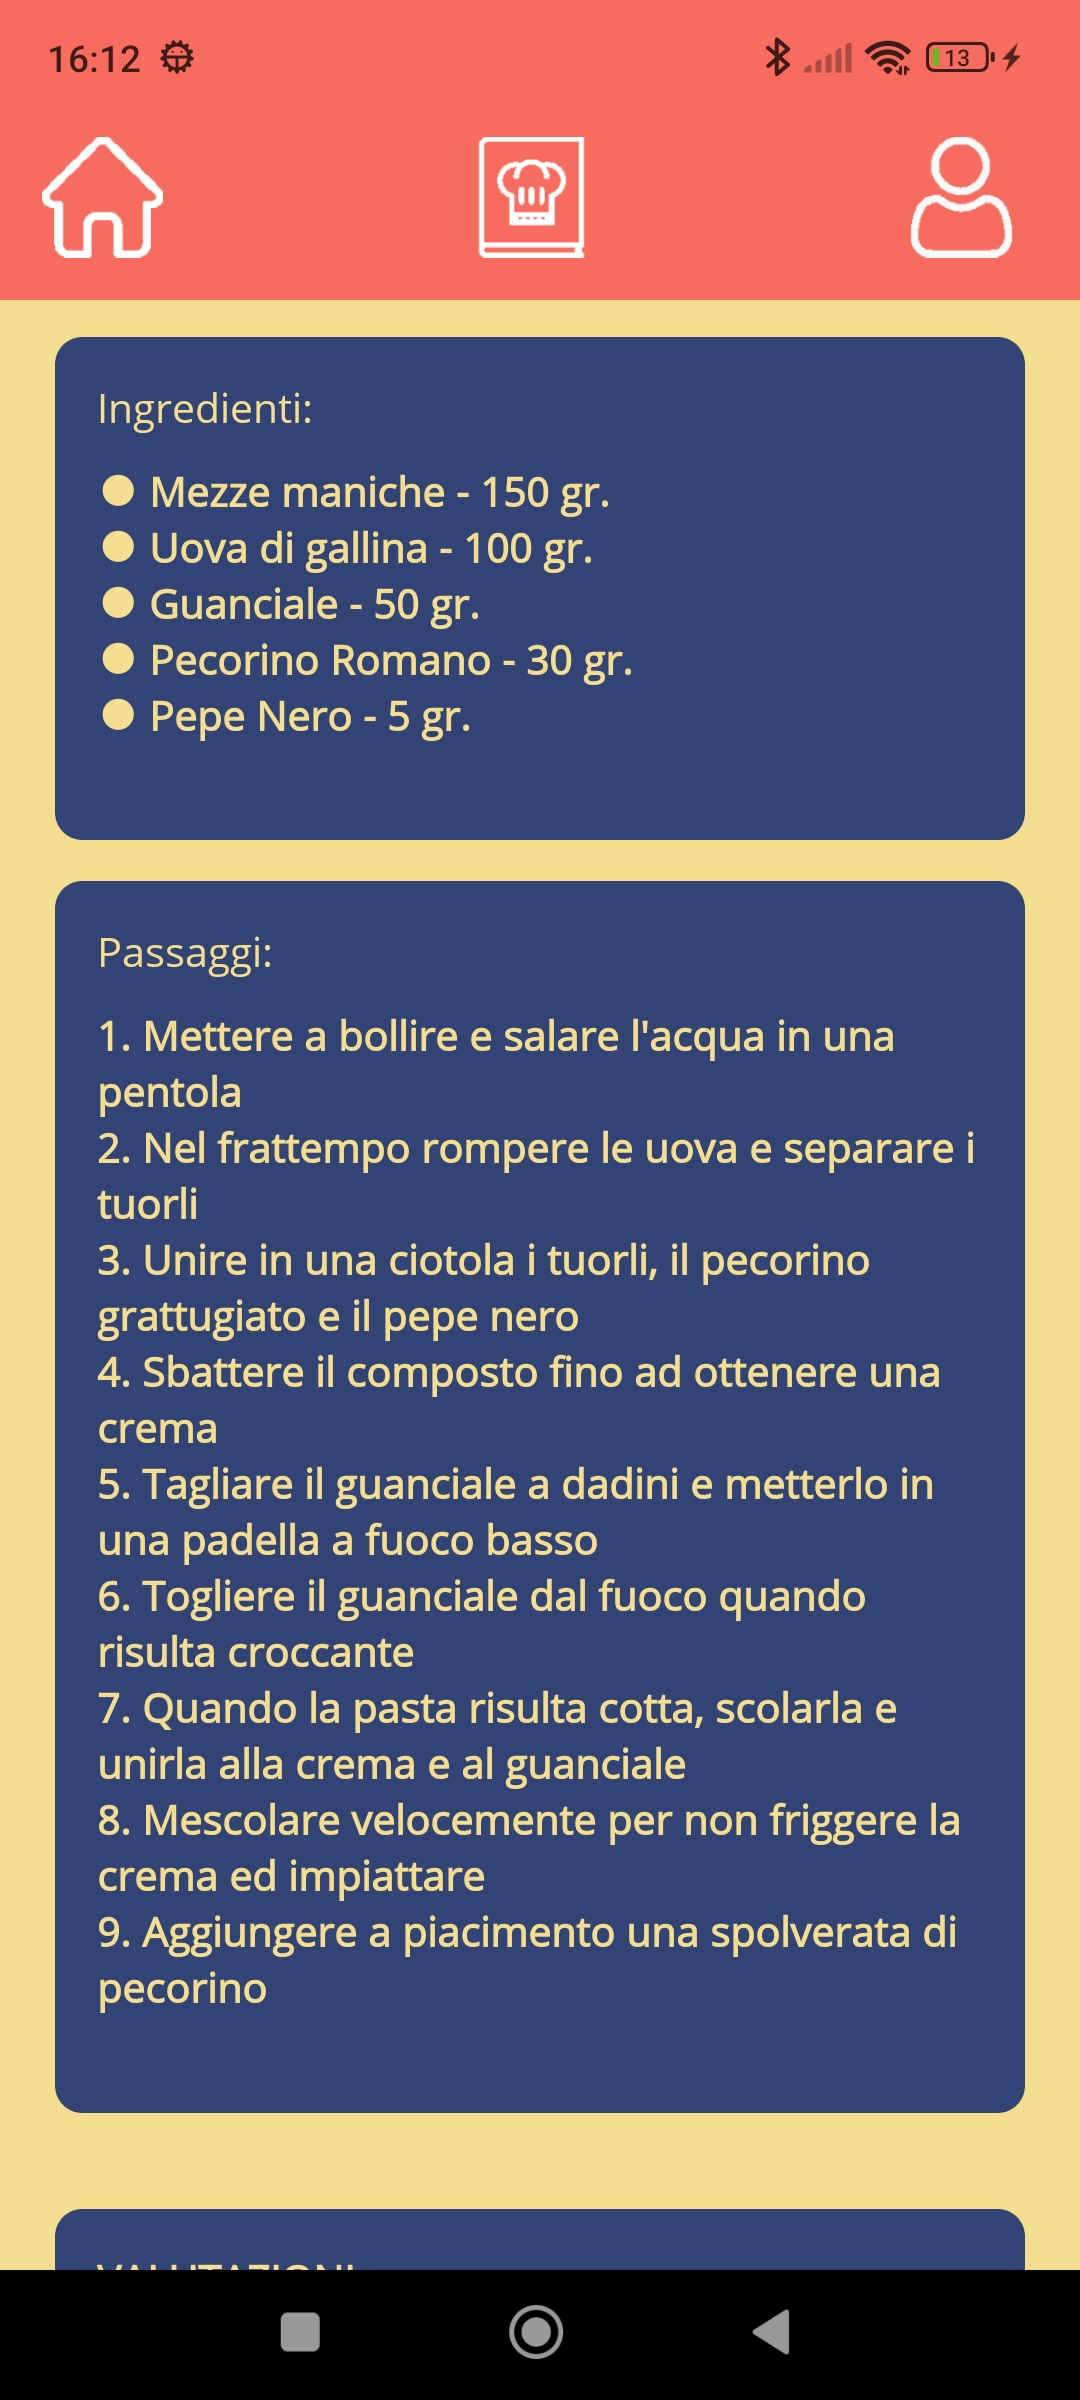
\includegraphics[width=0.9\linewidth]{app_images/RecipePage2.jpg}
    \end{minipage}
\end{figure}
\\In questa pagina l'utente potrà visualizzare tutte le informazioni della ricetta come la descrizione, gli ingredienti e i passaggi.
Inoltre potrà aggiungere la ricetta ai preferiti clickando sul pulsante con il cuore e potrà valutare la ricetta con un voto positivo (\colorbox{LimeGreen}{\textbf{Lime}}) o negativo (\colorbox{Tan}{\textbf{Cipolla}}).
In fondo alla pagina l'utente troverà la sezione delle valutazioni dove compariranno tutte le valutazioni degli utenti e l'utente potrà aggiungere un commento alla valutazione effettuata in precedenza.
\\\\\\Nella pagina della singola collezione/dieta, invece, si ha inizialmente una sezione con le informazioni principali, seguita dagli stessi bottoni per le valutazioni come nella pagina delle ricette e la lista delle ricette contenute nella collezione/dieta.
In fondo alla pagina si ha la sezione delle valutazioni con la possibilità di inserire il commento come per le ricette, nella pagina di una dieta però il commento può essere inserito solo se si ha sbloccato l'obiettivo della categoria nutrizionale a cui appartiene la dieta.
\begin{figure}[h!]
    \begin{minipage}{.5\textwidth}
        \centering
        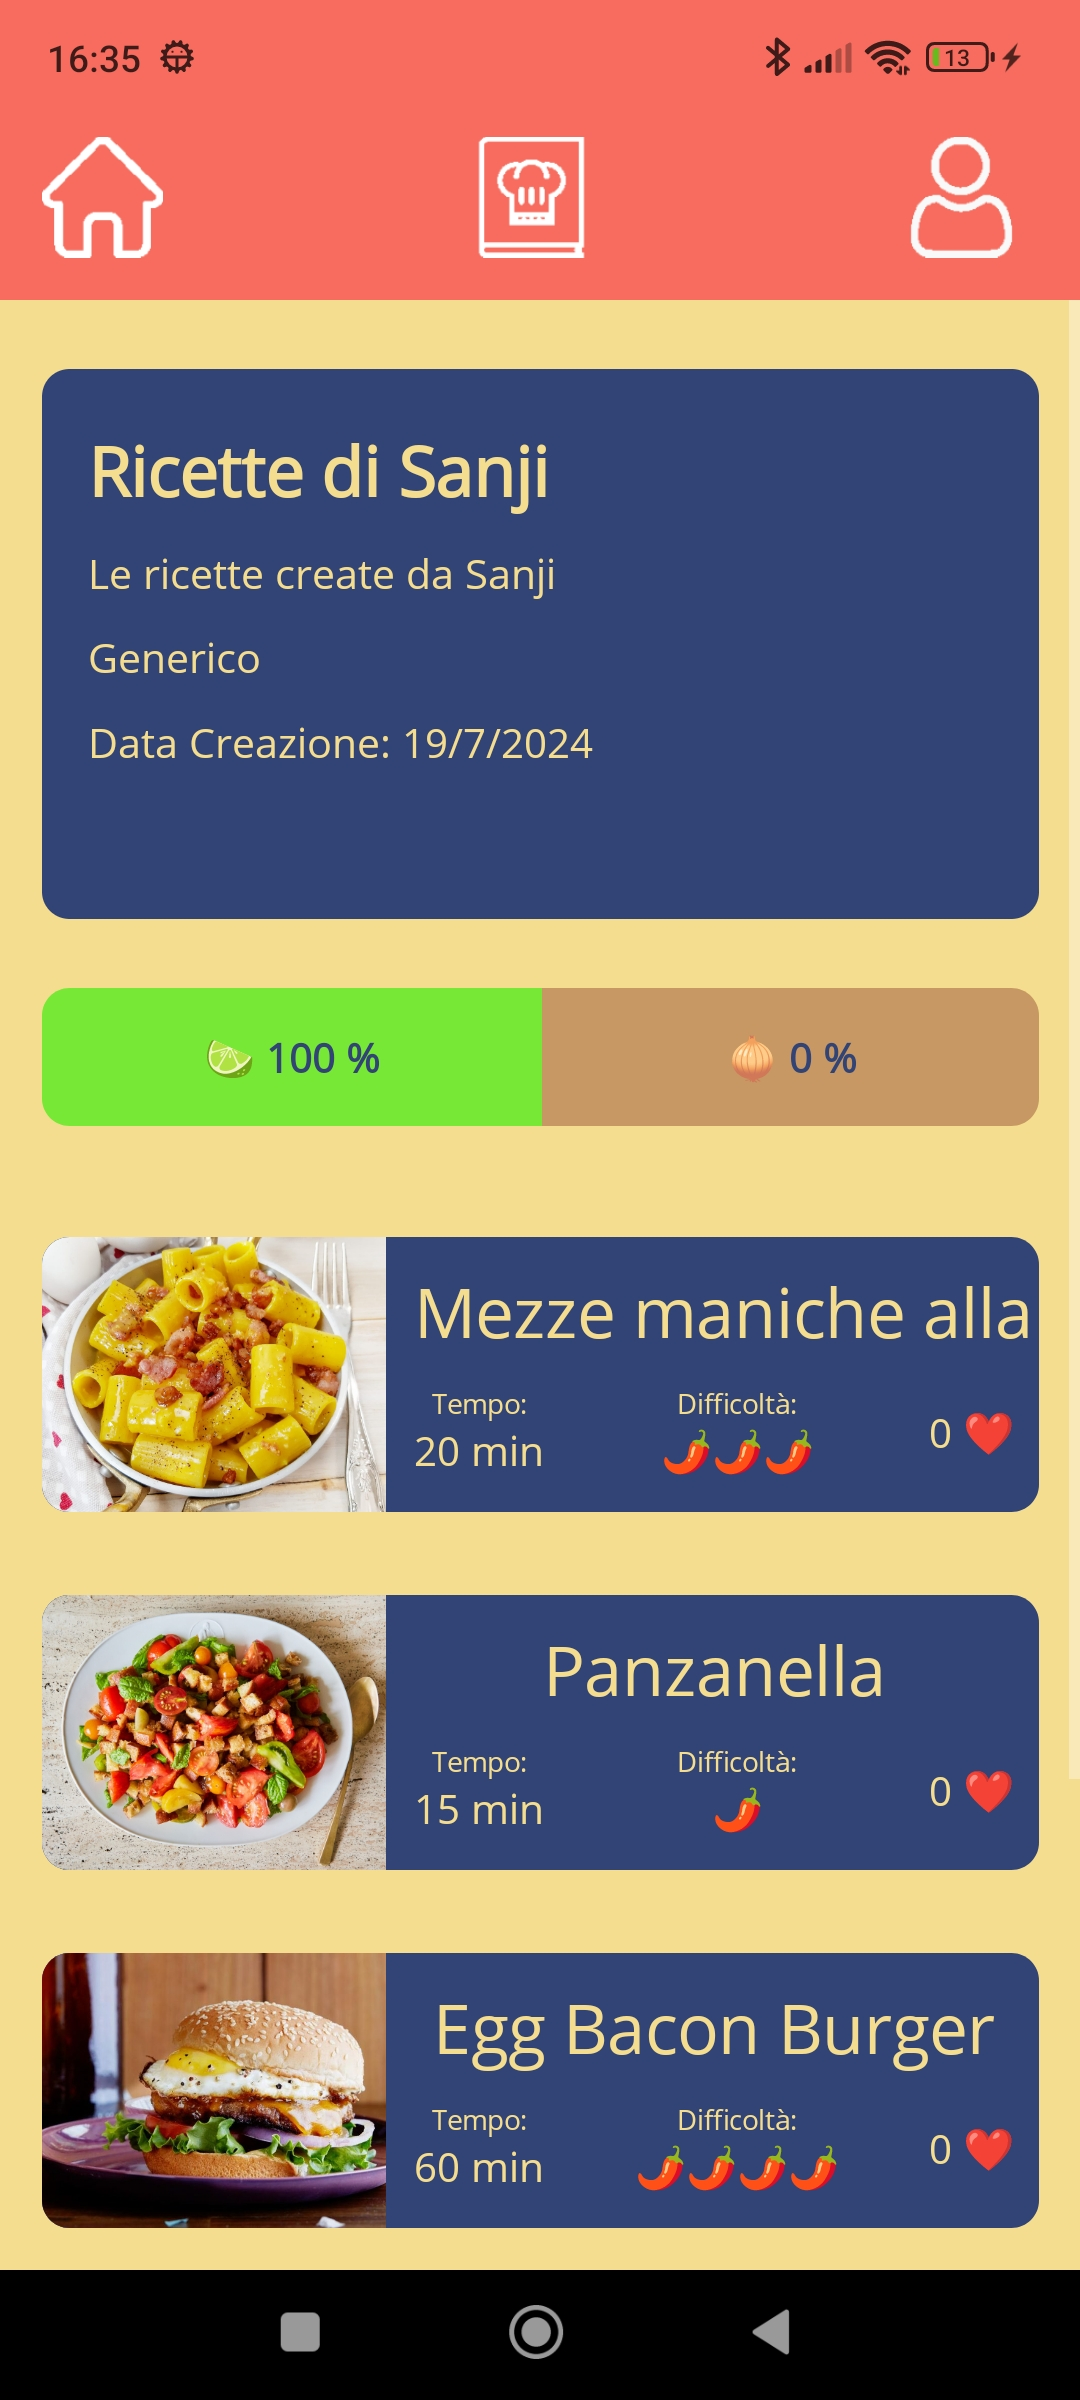
\includegraphics[width=0.9\linewidth]{app_images/CollectionPage.jpg}
    \end{minipage}
    \begin{minipage}{.5\textwidth}
        \centering
        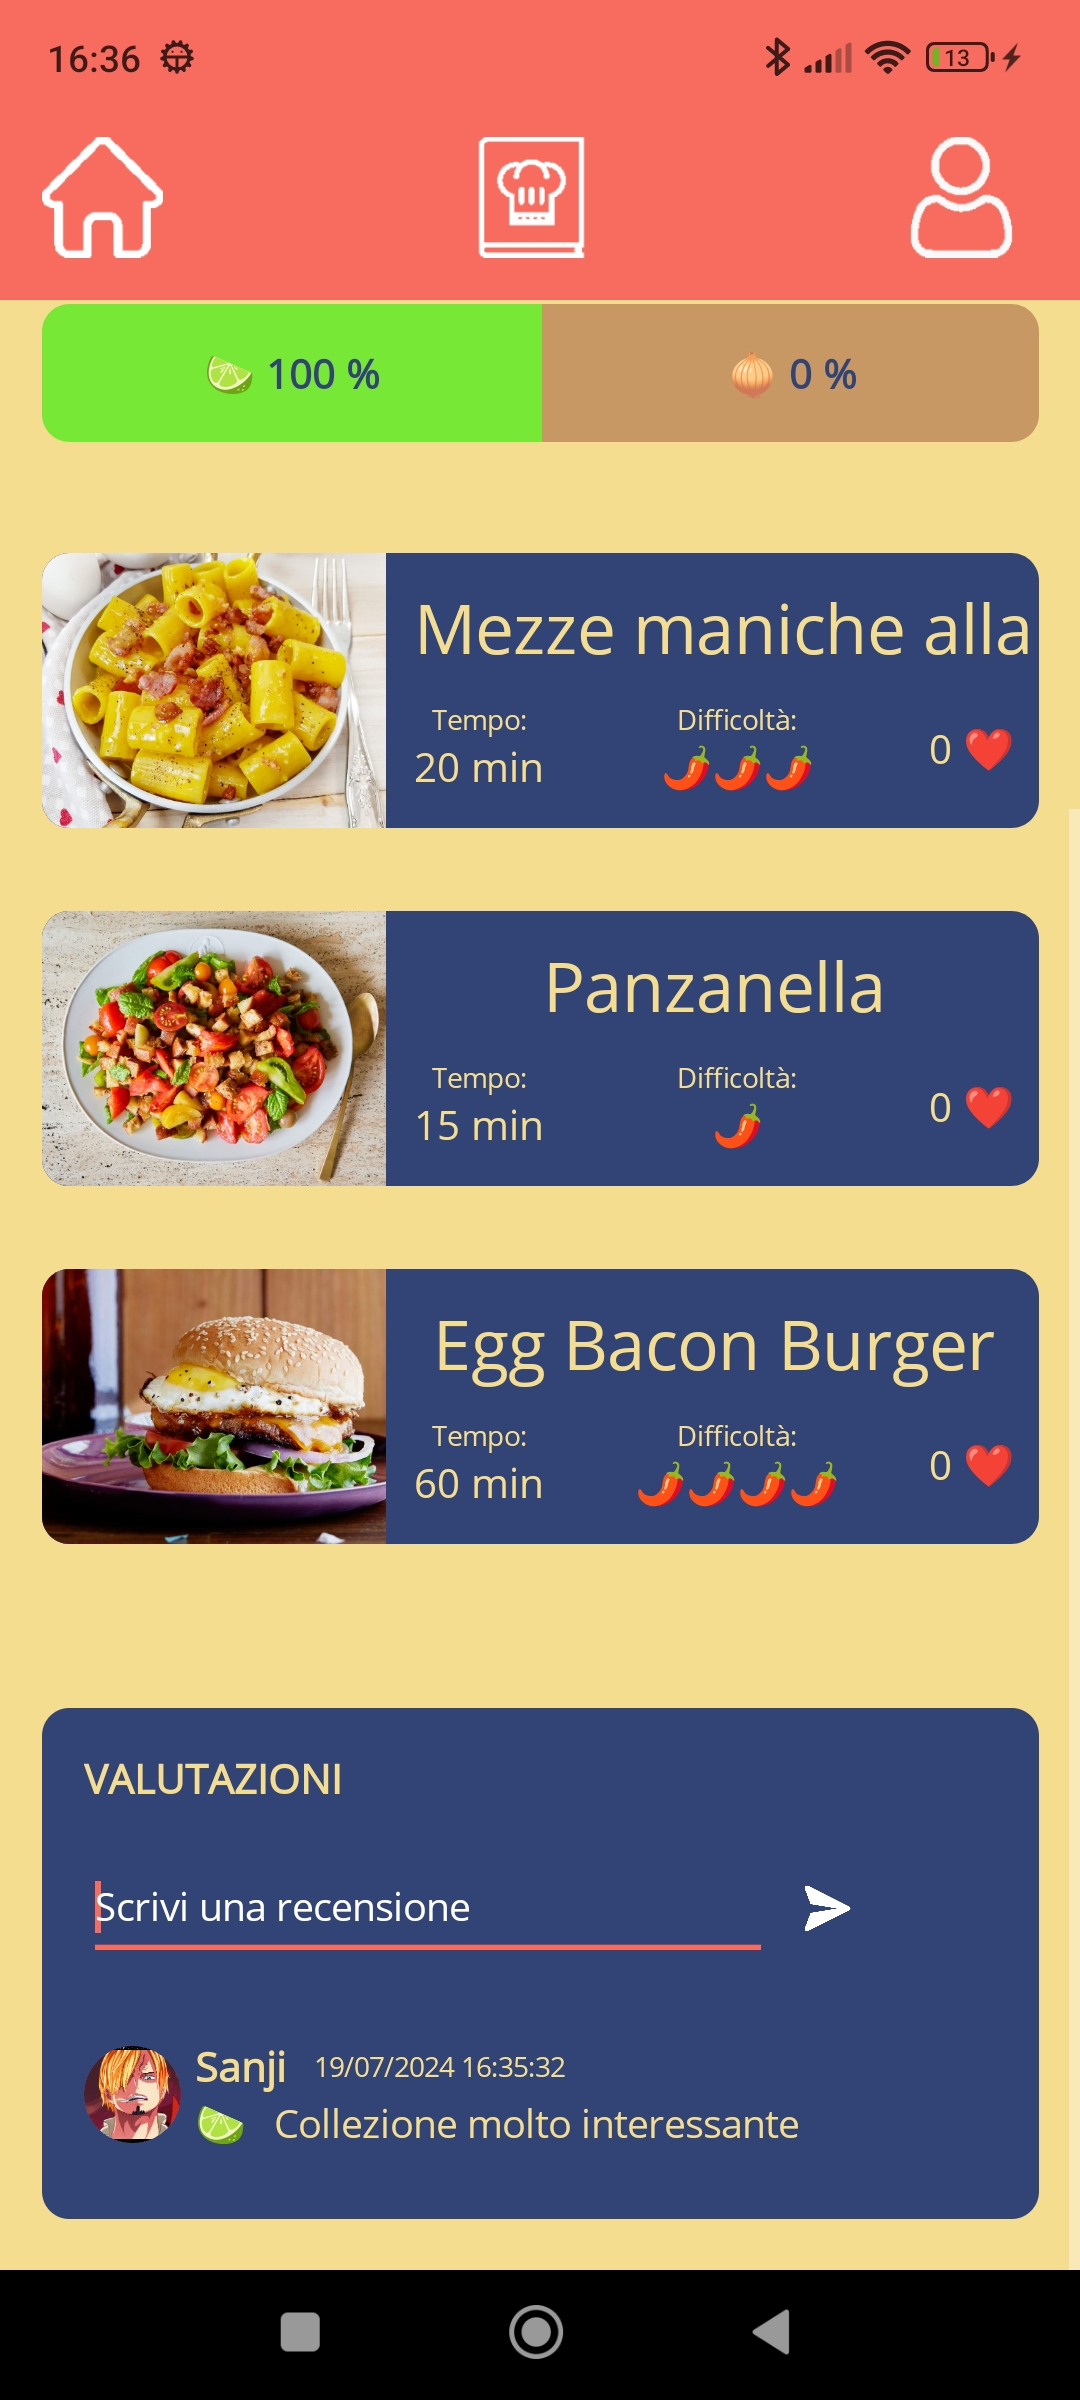
\includegraphics[width=0.9\linewidth]{app_images/CollectionPage2.jpg}
    \end{minipage}
\end{figure}
\\\\\\\\Tornando sul menu sovrastante di navigazione, clickando sull'icona a destra si andrà sulla propria pagina utente.
\\In questa pagina si ha la foto profilo inserita in fase di registrazione e il nome, seguiti da il tasto per effettuare il logout e i seguenti contatori delle statistiche dell'utente:
\begin{itemize}
    \item Numero di ricette create
    \item Numero di collezioni create
    \item Numero di recensioni create
    \item Numero di ricette aggiunte ai preferiti
    \item Numero di obiettivi ottenuti
\end{itemize}
Infine si hanno i pulsanti per la creazione di ricette e collezioni e una lista dove, al click di un contatore, compariranno gli elementi a cui fa riferimento quel contatore.
\begin{figure}[h!]
    \centering
    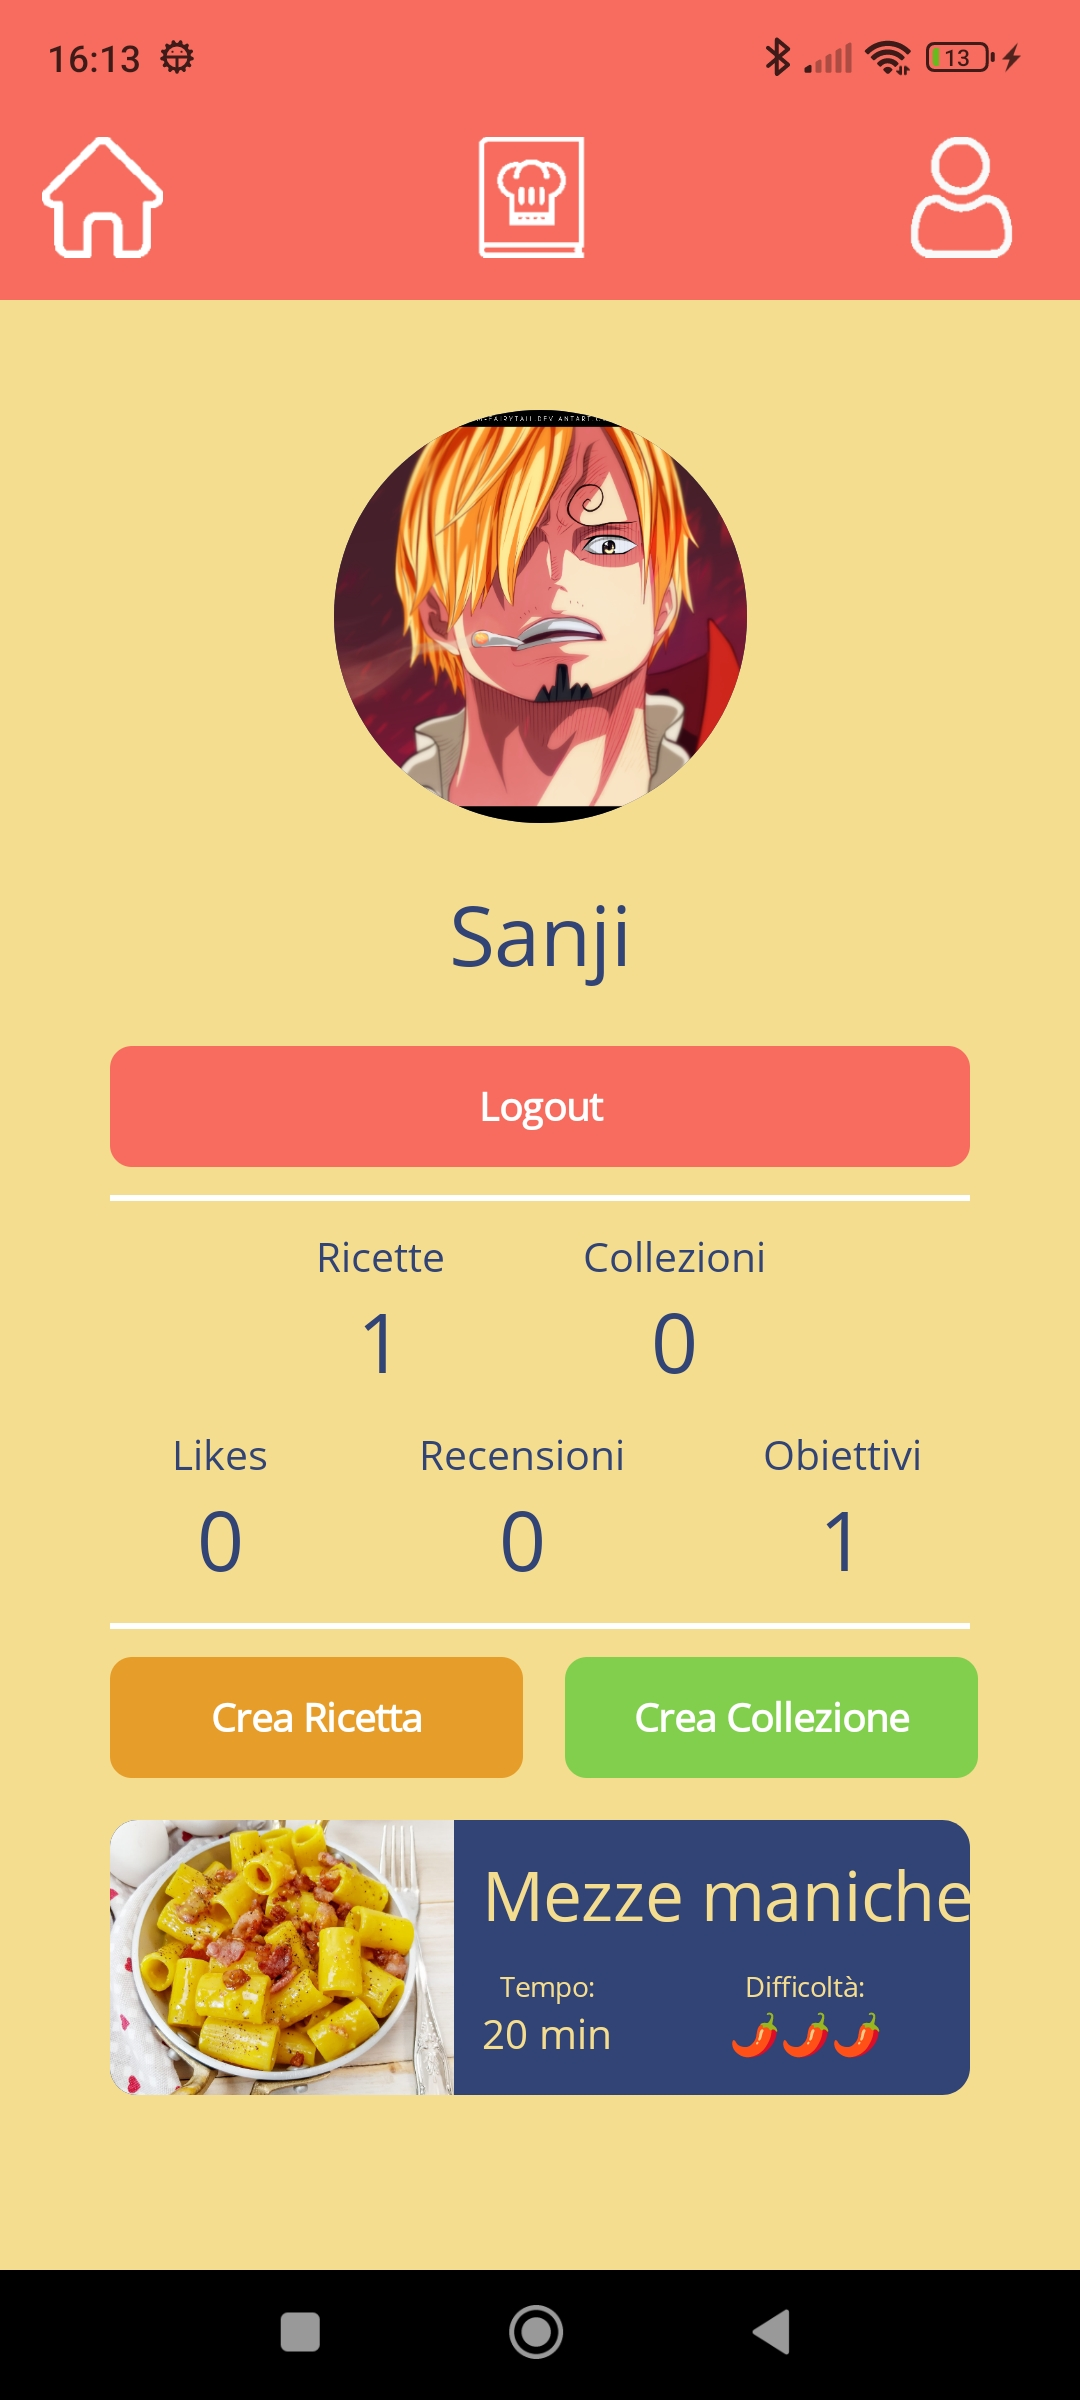
\includegraphics[width=0.4\linewidth]{app_images/UserPage.jpg}
\end{figure}
\\Clickando sul pulsante per la creazione di una ricetta comparirà la suddetta pagina con i vari campi da completare: 
\textbf{nome}, \textbf{descrizione}, \textbf{foto} (selezionandola dal proprio dispositivo), \textbf{lista dei passaggi} (scrivendo un passaggio alla volta e aggiungendolo alla lista), \textbf{difficoltà}, \textbf{tempo} e la \textbf{lista degli ingredienti} con la relativa quantità in grammi.\\
\begin{figure}[h!]
    \begin{minipage}{.5\textwidth}
        \centering
        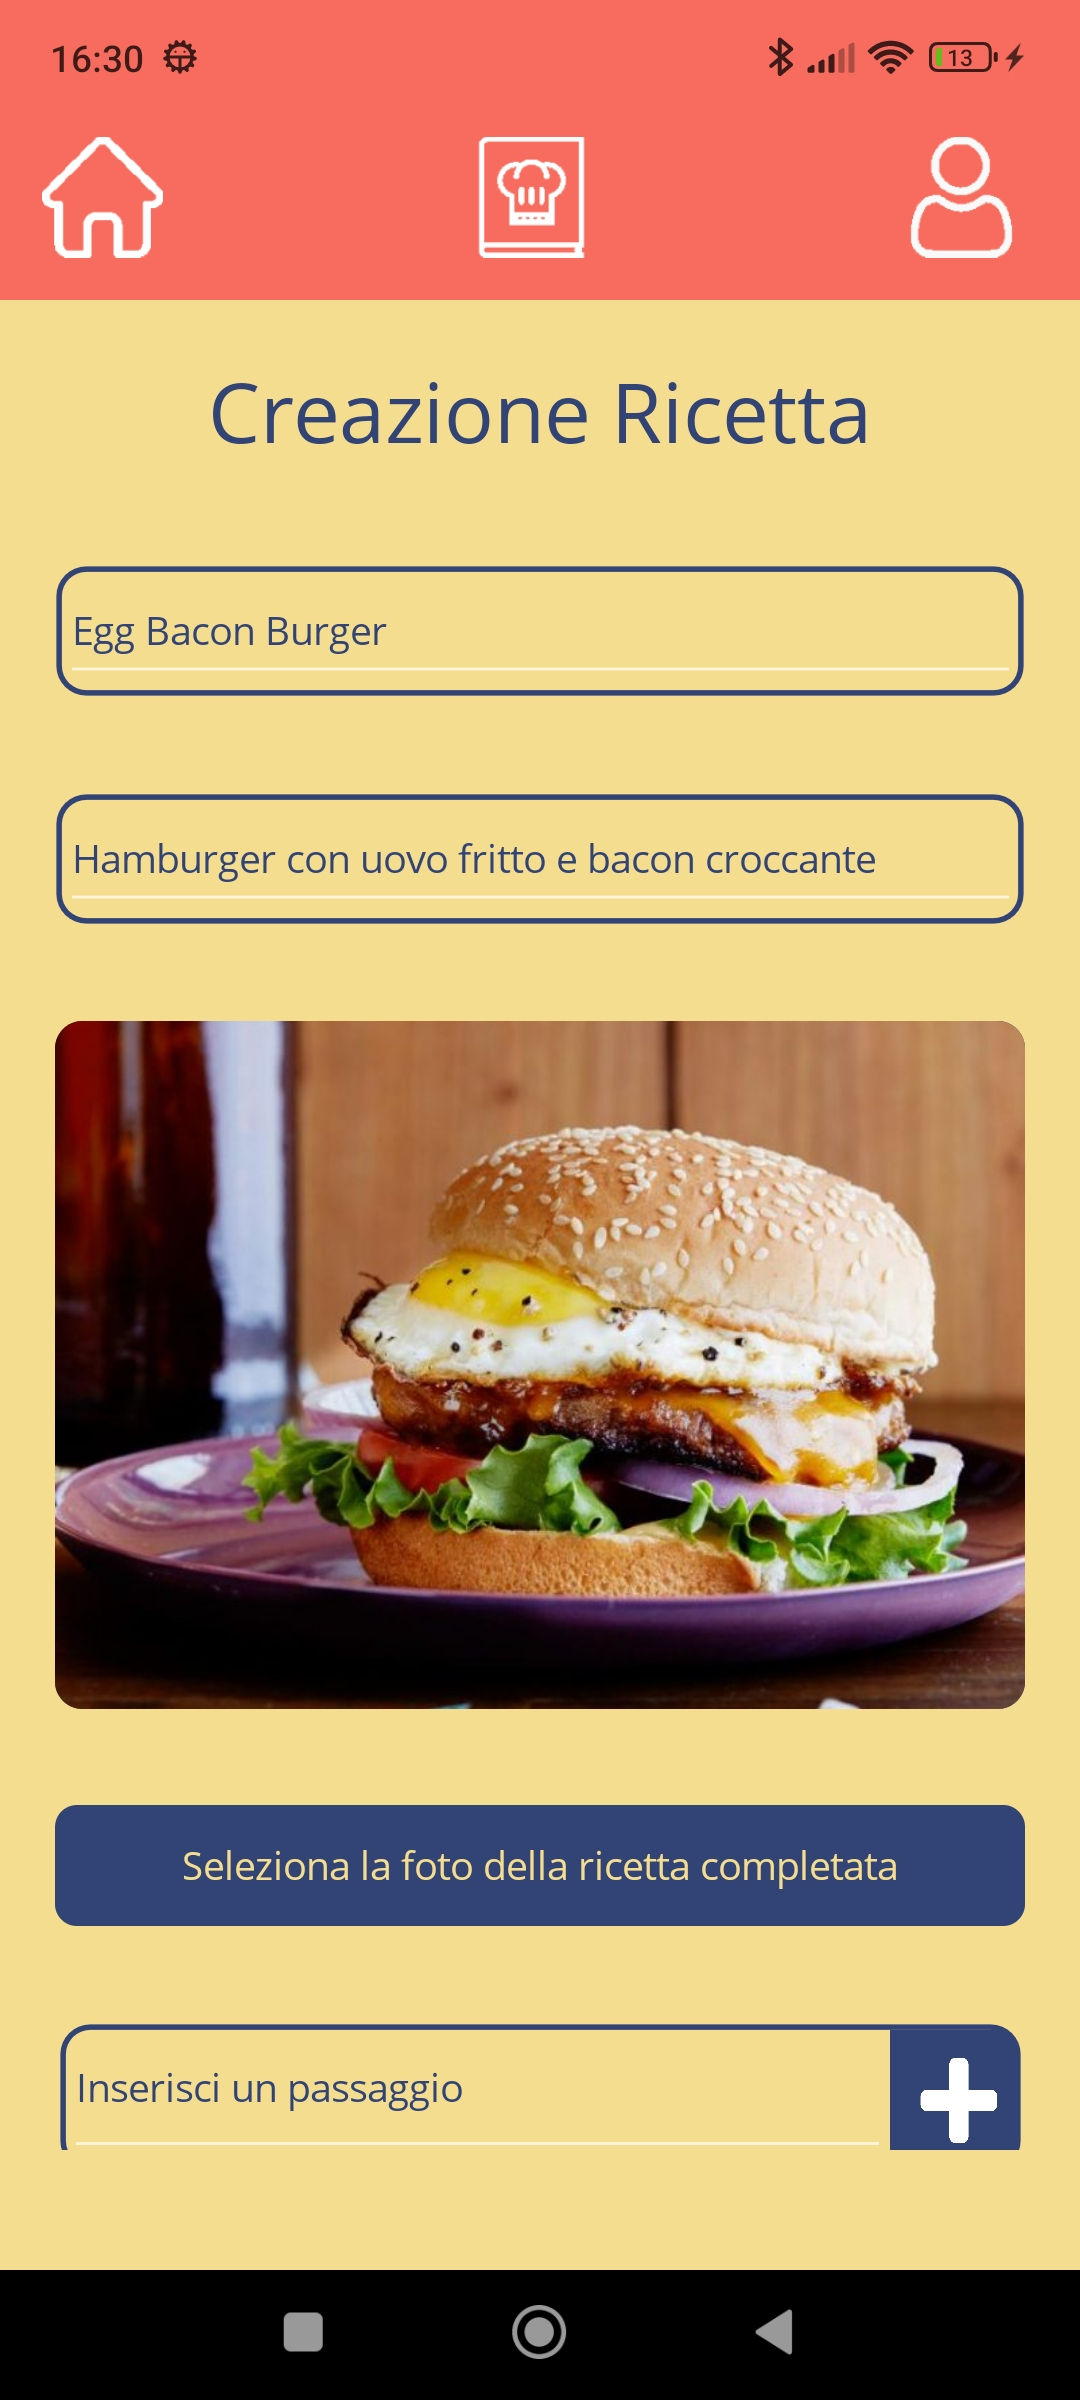
\includegraphics[width=0.9\linewidth]{app_images/RecipeCreation.jpg}
    \end{minipage}
    \begin{minipage}{.5\textwidth}
        \centering
        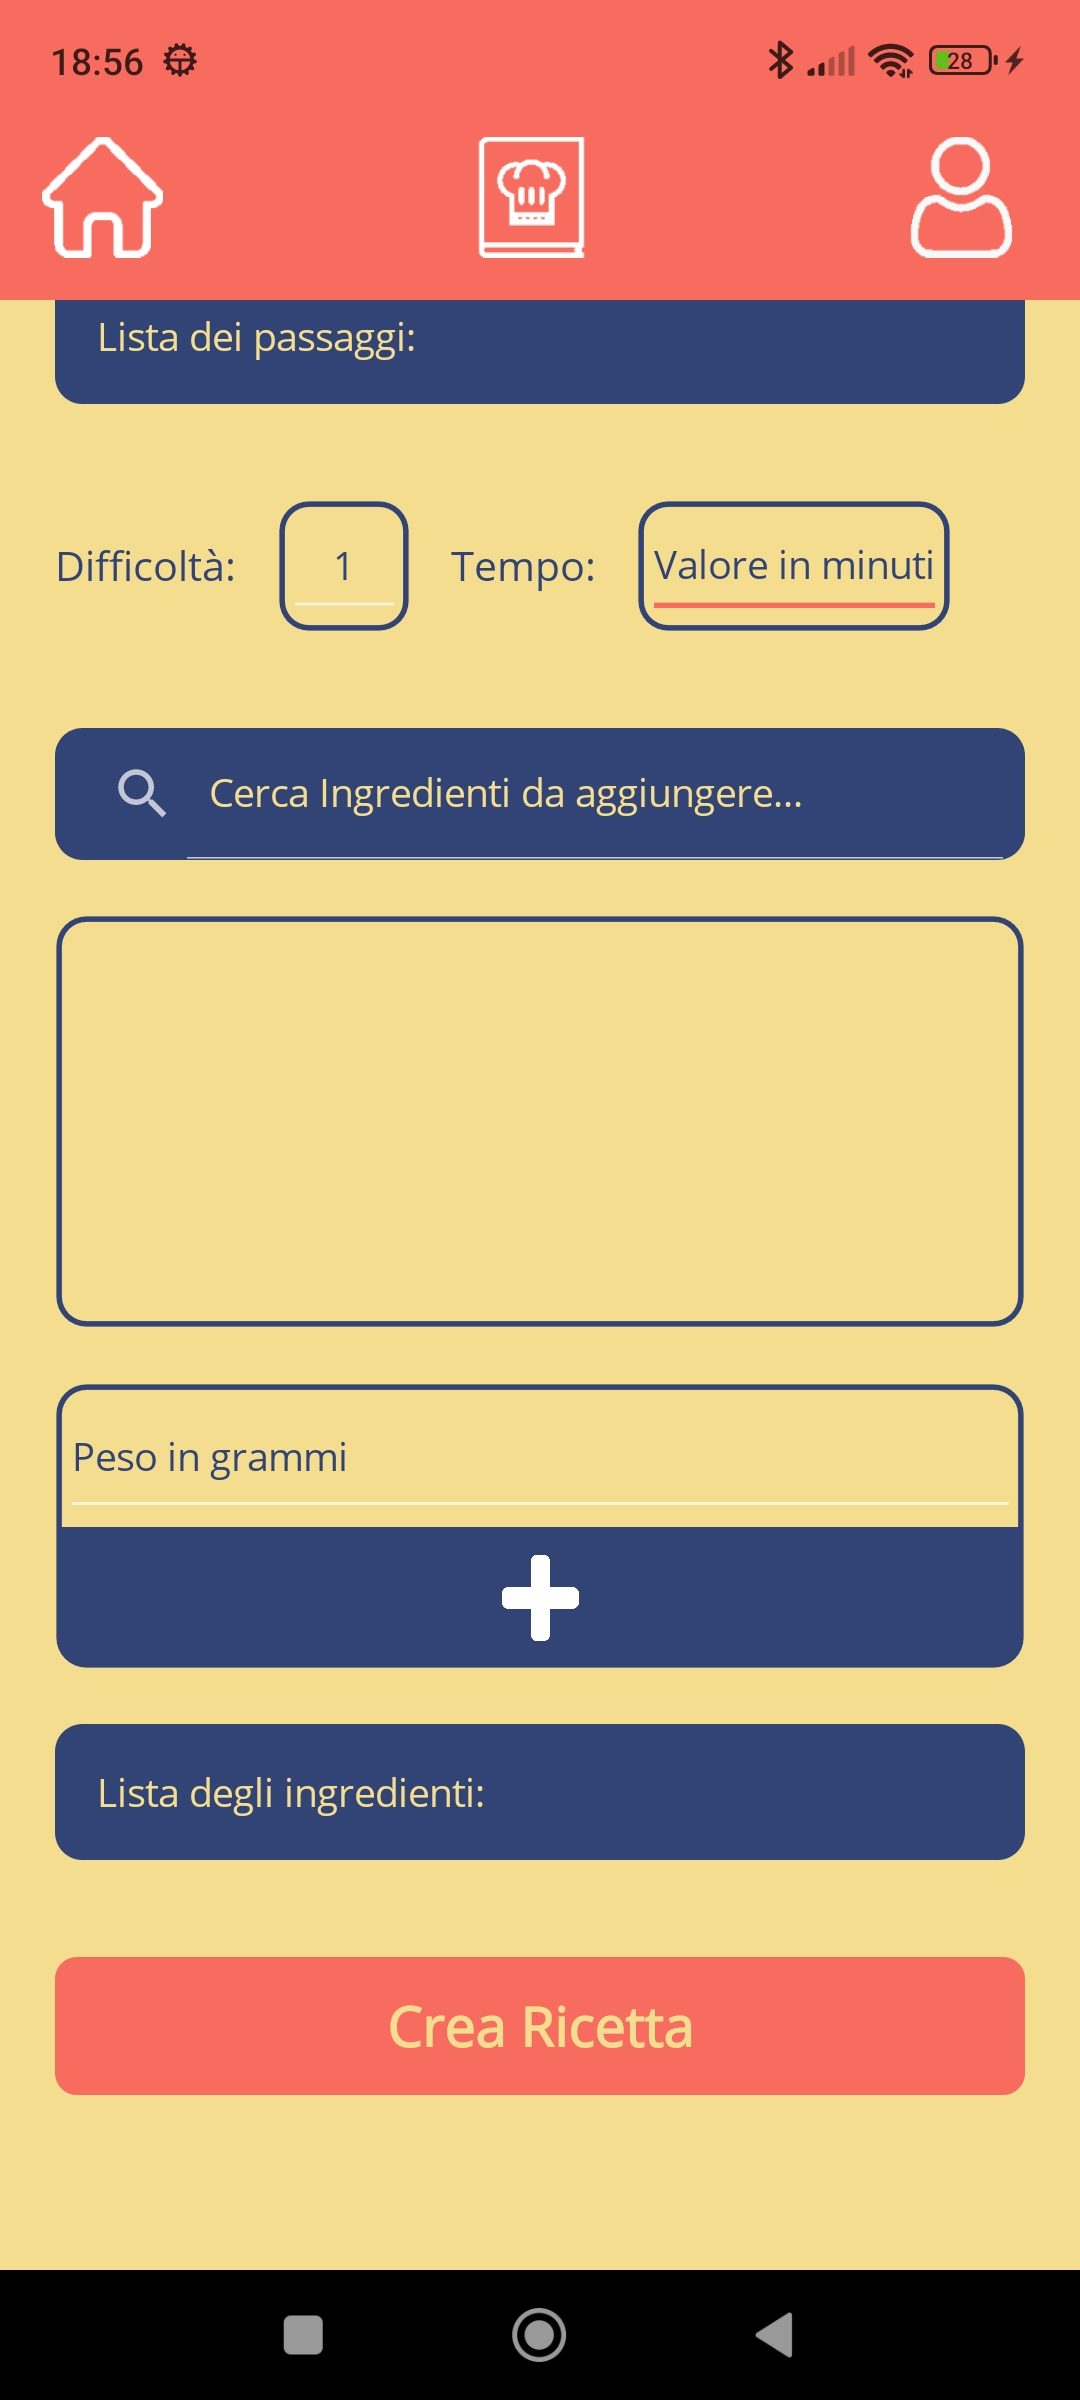
\includegraphics[width=0.9\linewidth]{app_images/RecipeCreation2.jpg}
    \end{minipage}
\end{figure}
\\\\\\\\\\\\\\Mentre clickando su quello per la creazione di collezioni/diete comparirà la pagina con i seguenti campi da completare:
\textbf{nome}, \textbf{descrizione}, checkbox per segnalare se si sta creando una \textbf{dieta} e scegliere la categoria nutrizionale e la \textbf{lista delle ricette} da aggiungere.
\begin{figure}[h!]
    \centering
    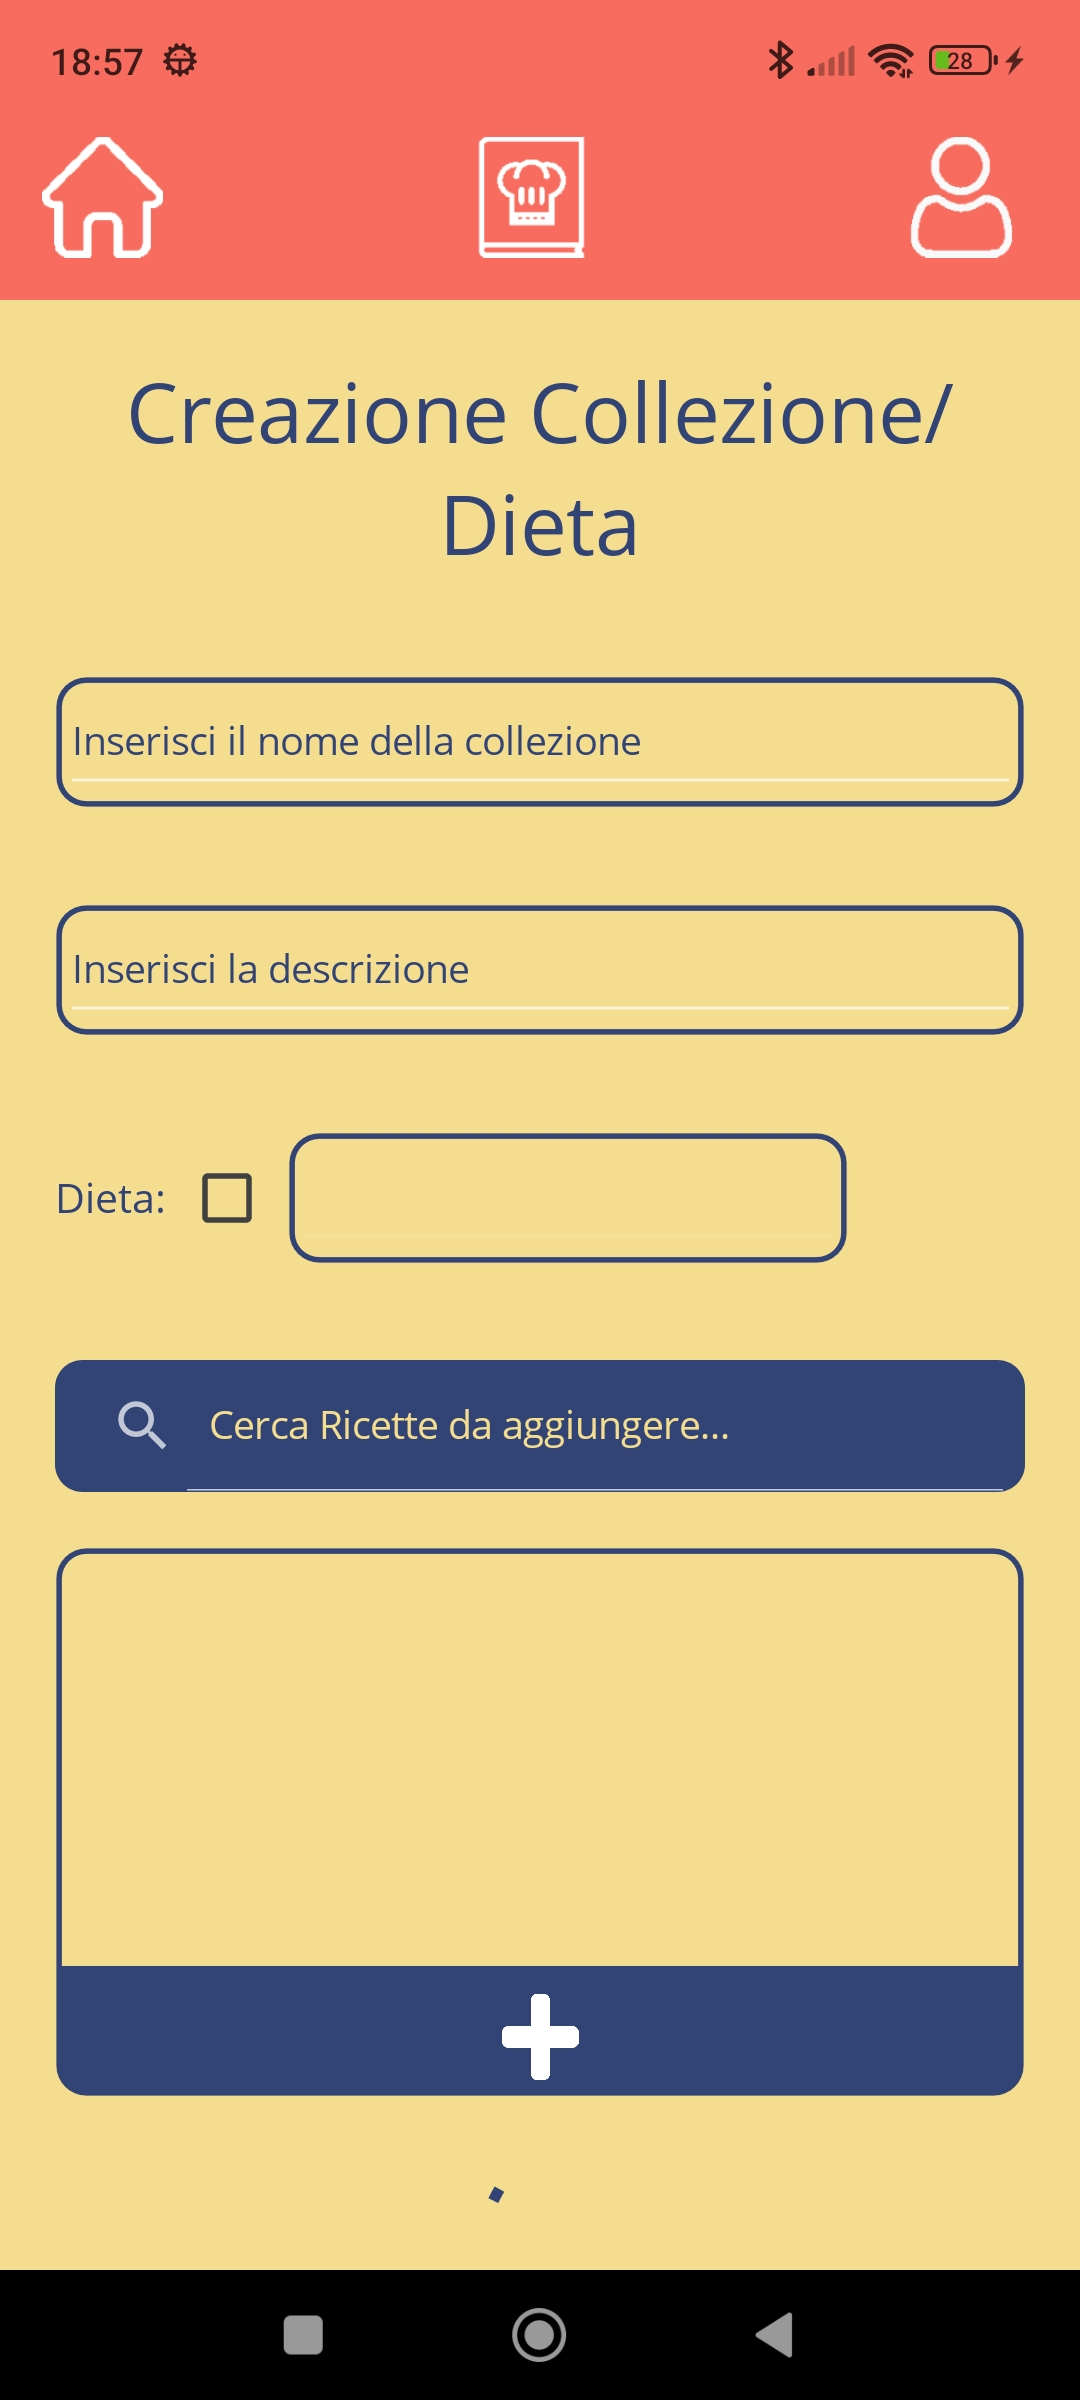
\includegraphics[width=0.5\linewidth]{app_images/CollectionCreation.jpg}
\end{figure}
\\\\\\\\\\\\Tutti i metodi che eseguono delle query sono contenuti dentro la classe MainViewModel che a sua volta utilizza un instanza globale di DBService per eseguire le query.
\section{Elenco delle query utilizzate}
\subsection{Query di selezione}
\begin{table}[h!]
    \centering
    \begin{tabular}{ |p{3in}|p{2in}| }
        \hline
        \scriptsize{\textbf{Nome}} & \scriptsize{\textbf{Operazione}} \\
        \hline
        \scriptsize{GetIngredients(int IdRicetta)} & \scriptsize{Restituisce tutti gli ingredienti appartenenti alla ricetta dell'ID dato} \\
        \hline
        \scriptsize{GetRecipes()} & \scriptsize{Restituisce le prime 10 ricette dotate del numero di like} \\
        \hline
        \scriptsize{GetRecipesByCollection(int IdCollezione)} & \scriptsize{Restituisce tutte le ricette appartenti alla collezione dell'ID dato} \\
        \hline
        \scriptsize{GetRecipesByDifficulty(int difficulty, string orderby)} & \scriptsize{Restituisce tutte le ricette con una data difficoltà e ordinate con il dato ordinamento} \\
        \hline
        \scriptsize{GetRecipesByTime(int time, string orderby)} & \scriptsize{Restituisce tutte le ricette con una dato tempo di preparazione e ordinate con il dato ordinamento} \\
        \hline
        \scriptsize{GetRecipesByUser(int userID)} & \scriptsize{Restituisce tutte le ricette appartenenti ad un dato utente} \\
        \hline
        \scriptsize{GetLikedRecipes(int userID)} & \scriptsize{Restituisce tutte le ricette aggiunte ai preferiti da un dato utente} \\
        \hline
        \scriptsize{GetReviewedRecipes(int userID)} & \scriptsize{Restituisce tutte le ricette valutate da un dato utente} \\
        \hline
        \scriptsize{GetRecipeById(int IdRicetta)} & \scriptsize{Restituisce la ricetta con il dato ID} \\
        \hline
        \scriptsize{GetCollectionById(int IdCollezione)} & \scriptsize{Restituisce la collezione con il dato ID compresa del nome della categoria nutrizionale a cui appartiene} \\
        \hline
        \scriptsize{GetCollectionsByUser(int userID)} & \scriptsize{Restituisce tutte le collezioni appartenenti ad un dato utente} \\
        \hline
        \scriptsize{GetCollectionsOrDiets(int Dieta)} & \scriptsize{Restituisce tutte le collezioni o diete, in base al parametro passato, comprese del nome della categoria nutrizionale a cui appartengono e della foto della ricetta con identificato meno recente che vi appartiene} \\
        \hline
        \scriptsize{GetUserById(int id)} & \scriptsize{Restituisce l'utente con ID dato compreso dei contatori di: ricette preferite, ricette valutate, ricette create, collezioni create e obiettivi ottenuti} \\
        \hline
        \scriptsize{GetMonthRecipes()} & \scriptsize{Restituisce le 3 ricette con più like} \\
        \hline
    \end{tabular}
\end{table}
\begin{table}[h!]
    \centering
    \begin{tabular}{ |p{3in}|p{2in}| }
        \hline
        \scriptsize{\textbf{Nome}} & \scriptsize{\textbf{Operazione}} \\
        \hline
        \scriptsize{GetNutritionalCategories(int IdRicetta)} & \scriptsize{Restituisce tutte le categorie nutrizionali a cui appartengono gli ingredienti di una ricetta} \\
        \hline
        \scriptsize{GetUnlockedNutritionalCategories()} & \scriptsize{Restituisce le categorie nutrizionali sbloccate dall'utente attraverso gli obiettivi} \\
        \hline
        \scriptsize{GetRatingsCountGroupByVoto(int id, bool isRecipe)} & \scriptsize{Restituisce il numero di voti positivi e negativi di una ricetta o di una collezione} \\
        \hline
        \scriptsize{GetRatingsById(int id, bool isRecipe)} & \scriptsize{Restituisce le valutazioni di una ricetta o di una collezione comprese dei nomi degli utenti e delle foto profilo} \\
        \hline
        \scriptsize{GetSearchedRecipes(string name, int IdCategoria)} & \scriptsize{Restituisce tutte le ricette con nome simile a quello dato e con tutti gli ingredienti appartenenti alla categoria nutrizionale data} \\
        \hline
        \scriptsize{GetSearchedIngredients(string text)} & \scriptsize{Restituisce tutti gli ingredienti con nome simile a quello dato} \\
        \hline
        \scriptsize{GetNutritionalCategories()} & \scriptsize{Restituisce tutte le categorie nutrizionali} \\
        \hline
        \scriptsize{GetFilteredRecipes(string difficulty, string time, string orderby, string category, string text)} & \scriptsize{Restituisce le ricette filtrate per difficoltà, tempo di preparazione, categoria nutrizionale degli ingredienti, nome e le ordina in base all'ordinamento dato} \\
        \hline
        \scriptsize{GetInsertedRecipeId()} & \scriptsize{Restituisce l'ID dell'ultima ricetta inserita dall'utente corrente} \\
        \hline
        \scriptsize{GetInsertedCollectionId()} & \scriptsize{Restituisce l'ID dell'ultima collezione inserita dall'utente corrente} \\
        \hline
        \scriptsize{CanUserLogin(string email, string password)} & \scriptsize{Restituisce un booleano in base al numero di occorrenze nella tabella utente con email e password pari a quelle date (0 = false)} \\
        \hline
        \scriptsize{GetLoggedUserId(string email)} & \scriptsize{Restituisce l'ID dell'utente che ha l'email pari a quella data} \\
        \hline
        \scriptsize{CanUserRegister(string email)} & \scriptsize{Restituisce un booleano in base al numero di occorrenze nella tabella utente con email pari a quella data (0 = true)} \\
        \hline
        \scriptsize{IsRecipeLikedByUser(int IdRicetta)} & \scriptsize{Restituisce un booleano in base al numero di occorrenze nella tabella likes ID della ricetta pari a quella dato (0 = false)} \\
        \hline
        \scriptsize{GetFilteredCollections(string text, string difficulty, string date, string orderby, string recipeNumber, int dieta, string nutritionalCategory)} & \scriptsize{Restituisce le collezioni o diete filtrate per difficoltà, data di creazione, categoria nutrizionale, nome, numero di ricette e le ordina in base all'ordinamento dato} \\
        \hline
        \scriptsize{GetObjectives(int IdUtente)} & \scriptsize{Restituisce gli obiettivi dell'utente corrente} \\
        \hline
    \end{tabular}
\end{table}
\subsection{Query di inserimento, aggiornamento e\\ rimozione}
\begin{table}[h!]
    \centering
    \begin{tabular}{ |p{3in}|p{2in}| }
        \hline
        \scriptsize{InsertRating(List〈Tuple〈string, object〉〉 rating, bool isRecipe)} & \scriptsize{Inserisce una valutazione su una ricetta o su una collezione da parte dell'utente corrente. Se l'elemento è già stato valutato e la valutazione da voler inserire è l'opposto di quella corrente, verrà prima eliminata la vecchia valutazione e poi verrà inserita quella attuale} \\
        \hline
        \scriptsize{InsertNewRecipe(List〈Tuple〈string, object〉〉 recipe)} & \scriptsize{Inserisce una nuova ricetta da parte dell'utente corrente} \\
        \hline
        \scriptsize{InsertRecipeIngredient(List〈Tuple〈string, object〉〉 ingredientRecipe)} & \scriptsize{Collega gli ingredienti ad una ricetta appena creata con i relativi pesi} \\
        \hline
        \scriptsize{InsertNewCollection(List〈Tuple〈string, object〉〉 collection)} & \scriptsize{Inserisce una nuova collezione da parte dell'utente corrente} \\
        \hline
        \scriptsize{InsertCollectionRecipe(List〈Tuple〈string, object〉〉 recipeCollection)} & \scriptsize{Collega le ricette ad una collezione appena creata} \\
        \hline
        \scriptsize{RegisterUser(List<Tuple<string, object>> userData)} & \scriptsize{Inserisce un nuovo utente} \\
        \hline
        \scriptsize{InsertReviewIfRatedByUser(int id, string comment, bool isRecipe)} & \scriptsize{Aggiorna, se esistente, una valutazione su una ricetta o su una collezione, inserendo il commento scritto dall'utente corrente} \\
        \hline
        \scriptsize{GiveRegisterObjective()} & \scriptsize{Sblocca all'utente che si è appena registrato l'obiettivo iniziale per la registrazione} \\
        \hline
        \scriptsize{AddOrRemoveRecipeFromLiked(int IdRicetta)} & \scriptsize{Aggiunge o rimuove dai preferiti dell'utente corrente una ricetta in base allo stato attuale} \\
        \hline
    \end{tabular}
\end{table}
\end{document}
